\documentclass[a4paper]{book}
\usepackage{makeidx}
\usepackage{natbib}
\usepackage{graphicx}
\usepackage{multicol}
\usepackage{float}
\usepackage{listings}
\usepackage{color}
\usepackage{ifthen}
\usepackage[table]{xcolor}
\usepackage{textcomp}
\usepackage{alltt}
\usepackage{ifpdf}
\ifpdf
\usepackage[pdftex,
            pagebackref=true,
            colorlinks=true,
            linkcolor=blue,
            unicode
           ]{hyperref}
\else
\usepackage[ps2pdf,
            pagebackref=true,
            colorlinks=true,
            linkcolor=blue,
            unicode
           ]{hyperref}
\usepackage{pspicture}
\fi
\usepackage[utf8]{inputenc}
\usepackage{mathptmx}
\usepackage[scaled=.90]{helvet}
\usepackage{courier}
\usepackage{sectsty}
\usepackage[titles]{tocloft}
\usepackage{doxygen}
\lstset{language=C++,inputencoding=utf8,basicstyle=\footnotesize,breaklines=true,breakatwhitespace=true,tabsize=4,numbers=left }
\makeindex
\setcounter{tocdepth}{3}
\renewcommand{\footrulewidth}{0.4pt}
\renewcommand{\familydefault}{\sfdefault}
\hfuzz=15pt
\setlength{\emergencystretch}{15pt}
\hbadness=750
\tolerance=750
\begin{document}
\hypersetup{pageanchor=false,citecolor=blue}
\begin{titlepage}
\vspace*{7cm}
\begin{center}
{\Large \-S\-Y\-M\-M\-E\-T\-R\-Y }\\
\vspace*{1cm}
{\large \-Generated by Doxygen 1.7.6.1}\\
\vspace*{0.5cm}
{\small Thu Feb 9 2012 22:35:46}\\
\end{center}
\end{titlepage}
\clearemptydoublepage
\pagenumbering{roman}
\tableofcontents
\clearemptydoublepage
\pagenumbering{arabic}
\hypersetup{pageanchor=true,citecolor=blue}
\chapter{\-E\-N\-G\-I\-N\-E}
\label{index}\hypertarget{index}{}\begin{DoxyAuthor}{Author}
A\-N\-D\-R\-E\-I M\-I\-L\-E\-A
\end{DoxyAuthor}
Computational library(numerical recipes, symbolic computation, etc). 
\chapter{\-Namespace \-Index}
\section{Namespace List}
Here is a list of all documented namespaces with brief descriptions\-:\begin{DoxyCompactList}
\item\contentsline{section}{\hyperlink{namespaceengine}{engine} }{\pageref{namespaceengine}}{}
\end{DoxyCompactList}

\chapter{\-Class \-Index}
\section{Class Hierarchy}
This inheritance list is sorted roughly, but not completely, alphabetically\-:\begin{DoxyCompactList}
\item \contentsline{section}{Addition}{\pageref{classAddition}}{}
\item \contentsline{section}{tree\-:\-:btree\-\_\-iterator$<$ T, N $>$}{\pageref{classtree_1_1btree__iterator}}{}
\begin{DoxyCompactList}
\item \contentsline{section}{tree\-:\-:btree\-\_\-inorder\-\_\-iterator$<$ T, N $>$}{\pageref{classtree_1_1btree__inorder__iterator}}{}
\item \contentsline{section}{tree\-:\-:btree\-\_\-postorder\-\_\-iterator$<$ T, N $>$}{\pageref{classtree_1_1btree__postorder__iterator}}{}
\item \contentsline{section}{tree\-:\-:btree\-\_\-preorder\-\_\-iterator$<$ T, N $>$}{\pageref{classtree_1_1btree__preorder__iterator}}{}
\end{DoxyCompactList}
\item \contentsline{section}{tree\-:\-:btree\-\_\-iterator$<$ T, btree\-\_\-threaded\-\_\-node$<$ T $>$ $>$}{\pageref{classtree_1_1btree__iterator_3_01T_00_01btree__threaded__node_3_01T_01_4_01_4}}{}
\begin{DoxyCompactList}
\item \contentsline{section}{tree\-:\-:btree\-\_\-inorder\-\_\-iterator$<$ T, btree\-\_\-threaded\-\_\-node$<$ T $>$ $>$}{\pageref{classtree_1_1btree__inorder__iterator_3_01T_00_01btree__threaded__node_3_01T_01_4_01_4}}{}
\end{DoxyCompactList}
\item \contentsline{section}{tree\-:\-:btree\-\_\-node$<$ T $>$}{\pageref{structtree_1_1btree__node}}{}
\item \contentsline{section}{tree\-:\-:btree\-\_\-threaded\-\_\-node$<$ T $>$}{\pageref{structtree_1_1btree__threaded__node}}{}
\item \contentsline{section}{tree\-:\-:c\-Binary\-Rep$<$ T $>$}{\pageref{classtree_1_1cBinaryRep}}{}
\item \contentsline{section}{tree\-:\-:c\-Binary\-Tree$<$ T, R\-E\-P $>$}{\pageref{classtree_1_1cBinaryTree}}{}
\item \contentsline{section}{c\-Cayley\-Grf$<$ G $>$}{\pageref{classcCayleyGrf}}{}
\item \contentsline{section}{c\-Cayley\-Grf$<$ G $>$\-:\-:c\-Colour\-Edges\-Vis$<$ E, Grf $>$}{\pageref{classcCayleyGrf_1_1cColourEdgesVis}}{}
\item \contentsline{section}{c\-Gen\-Rep$<$ T $>$}{\pageref{classcGenRep}}{}
\item \contentsline{section}{c\-Group$<$ T, group\-\_\-rep $>$}{\pageref{classcGroup}}{}
\item \contentsline{section}{c\-Group\-Elem$<$ T, Binary\-Op $>$}{\pageref{classcGroupElem}}{}
\item \contentsline{section}{c\-Group\-Relation}{\pageref{classcGroupRelation}}{}
\item \contentsline{section}{c\-Grp\-Lattice$<$ G $>$}{\pageref{classcGrpLattice}}{}
\item \contentsline{section}{c\-Homomorphism$<$ G1, G2 $>$}{\pageref{classcHomomorphism}}{}
\item \contentsline{section}{c\-Int\-Mod\-N\-Elem$<$ N $>$}{\pageref{classcIntModNElem}}{}
\item \contentsline{section}{Composition}{\pageref{classComposition}}{}
\item \contentsline{section}{c\-Perm\-Elem}{\pageref{classcPermElem}}{}
\item \contentsline{section}{c\-S\-L\-P\-Rep$<$ T $>$}{\pageref{classcSLPRep}}{}
\item \contentsline{section}{c\-Subgroup$<$ G $>$}{\pageref{classcSubgroup}}{}
\item \contentsline{section}{c\-Symmetric\-Rep$<$ T $>$}{\pageref{classcSymmetricRep}}{}
\item \contentsline{section}{tree\-:\-:c\-Threaded\-Rep$<$ T $>$}{\pageref{classtree_1_1cThreadedRep}}{}
\item \contentsline{section}{Factorial$<$ V\-A\-L $>$}{\pageref{structFactorial}}{}
\item \contentsline{section}{Factorial$<$ 0 $>$}{\pageref{structFactorial_3_010_01_4}}{}
\item \contentsline{section}{Multiplication}{\pageref{classMultiplication}}{}
\end{DoxyCompactList}

\chapter{\-Class \-Index}
\section{\-Class \-List}
\-Here are the classes, structs, unions and interfaces with brief descriptions\-:\begin{DoxyCompactList}
\item\contentsline{section}{\hyperlink{classengine_1_1cGroupGenCommand_1_1AddGrpGen}{engine\-::c\-Group\-Gen\-Command\-::\-Add\-Grp\-Gen} }{\pageref{classengine_1_1cGroupGenCommand_1_1AddGrpGen}}{}
\item\contentsline{section}{\hyperlink{classengine_1_1cCommand}{engine\-::c\-Command} }{\pageref{classengine_1_1cCommand}}{}
\item\contentsline{section}{\hyperlink{classengine_1_1cCommandCreator}{engine\-::c\-Command\-Creator$<$ C\-R\-E\-A\-T\-O\-R $>$} }{\pageref{classengine_1_1cCommandCreator}}{}
\item\contentsline{section}{\hyperlink{classengine_1_1cCommandQueue}{engine\-::c\-Command\-Queue} }{\pageref{classengine_1_1cCommandQueue}}{}
\item\contentsline{section}{\hyperlink{classengine_1_1cCreator}{engine\-::c\-Creator} }{\pageref{classengine_1_1cCreator}}{}
\item\contentsline{section}{\hyperlink{classengine_1_1cEstimator}{engine\-::c\-Estimator} }{\pageref{classengine_1_1cEstimator}}{}
\item\contentsline{section}{\hyperlink{classengine_1_1cGetElemCommand}{engine\-::c\-Get\-Elem\-Command} }{\pageref{classengine_1_1cGetElemCommand}}{}
\item\contentsline{section}{\hyperlink{classengine_1_1cGetSubgrpCommand}{engine\-::c\-Get\-Subgrp\-Command} }{\pageref{classengine_1_1cGetSubgrpCommand}}{}
\item\contentsline{section}{\hyperlink{classcGroupFactory}{c\-Group\-Factory} }{\pageref{classcGroupFactory}}{}
\item\contentsline{section}{\hyperlink{classengine_1_1cGroupGenCommand}{engine\-::c\-Group\-Gen\-Command} }{\pageref{classengine_1_1cGroupGenCommand}}{}
\item\contentsline{section}{\hyperlink{classcInterpreter}{c\-Interpreter} }{\pageref{classcInterpreter}}{}
\item\contentsline{section}{\hyperlink{classengine_1_1cLogger}{engine\-::c\-Logger} }{\pageref{classengine_1_1cLogger}}{}
\item\contentsline{section}{\hyperlink{classengine_1_1cResult}{engine\-::c\-Result} }{\pageref{classengine_1_1cResult}}{}
\item\contentsline{section}{\hyperlink{classcSerializer_3_01SymmGrpElem_00_01CONT_01_4}{c\-Serializer$<$ Symm\-Grp\-Elem, C\-O\-N\-T $>$} }{\pageref{classcSerializer_3_01SymmGrpElem_00_01CONT_01_4}}{}
\item\contentsline{section}{\hyperlink{classengine_1_1cSession}{engine\-::c\-Session} }{\pageref{classengine_1_1cSession}}{}
\item\contentsline{section}{\hyperlink{classengine_1_1cThreadPool}{engine\-::c\-Thread\-Pool} }{\pageref{classengine_1_1cThreadPool}}{}
\item\contentsline{section}{\hyperlink{classengine_1_1cVariantVisitor}{engine\-::c\-Variant\-Visitor} }{\pageref{classengine_1_1cVariantVisitor}}{}
\item\contentsline{section}{\hyperlink{structengine_1_1cGroupGenCommand_1_1group__type__}{engine\-::c\-Group\-Gen\-Command\-::group\-\_\-type\-\_\-} }{\pageref{structengine_1_1cGroupGenCommand_1_1group__type__}}{}
\end{DoxyCompactList}

\chapter{\-Namespace \-Documentation}
\hypertarget{namespaceengine}{\section{engine Namespace Reference}
\label{namespaceengine}\index{engine@{engine}}
}
\subsection*{Classes}
\begin{DoxyCompactItemize}
\item 
class \hyperlink{classengine_1_1cCommand}{c\-Command}
\item 
class \hyperlink{classengine_1_1cCommandCreator}{c\-Command\-Creator}
\item 
class \hyperlink{classengine_1_1cCommandQueue}{c\-Command\-Queue}
\item 
class \hyperlink{classengine_1_1cEstimator}{c\-Estimator}
\item 
class \hyperlink{classengine_1_1cGetCenterCommand}{c\-Get\-Center\-Command}
\item 
class \hyperlink{classengine_1_1cGetCGraphCommand}{c\-Get\-C\-Graph\-Command}
\item 
class \hyperlink{classengine_1_1cGetElemCommand}{c\-Get\-Elem\-Command}
\item 
class \hyperlink{classengine_1_1cGetMatExprCommand}{c\-Get\-Mat\-Expr\-Command}
\item 
class \hyperlink{classengine_1_1cGetRelCommand}{c\-Get\-Rel\-Command}
\item 
class \hyperlink{classengine_1_1cParamGrpGenParser}{c\-Param\-Grp\-Gen\-Parser}
\item 
class \hyperlink{classengine_1_1cGroupGenCommand}{c\-Group\-Gen\-Command}
\item 
class \hyperlink{classengine_1_1cLinAlgCommand}{c\-Lin\-Alg\-Command}
\item 
struct \hyperlink{structengine_1_1cMatrix}{c\-Matrix}
\item 
struct \hyperlink{structengine_1_1sLinFactor}{s\-Lin\-Factor}
\item 
struct \hyperlink{structengine_1_1sLinTerm}{s\-Lin\-Term}
\item 
struct \hyperlink{structengine_1_1sLinExpression}{s\-Lin\-Expression}
\item 
struct \hyperlink{structengine_1_1lin__expr__grammar}{lin\-\_\-expr\-\_\-grammar}
\item 
class \hyperlink{classengine_1_1cLinAlgParser}{c\-Lin\-Alg\-Parser}
\item 
class \hyperlink{classengine_1_1cVariantVisitor}{c\-Variant\-Visitor}
\item 
class \hyperlink{classengine_1_1cLogger}{c\-Logger}
\item 
class \hyperlink{classengine_1_1cSession}{c\-Session}
\item 
class \hyperlink{classengine_1_1cThreadPool}{c\-Thread\-Pool}
\end{DoxyCompactItemize}
\subsection*{Typedefs}
\begin{DoxyCompactItemize}
\item 
\hypertarget{namespaceengine_af1b349928e8ef52af7a7b83676140e9d}{typedef boost\-::unique\-\_\-lock\\*
$<$ boost\-::mutex $>$ {\bfseries lock\-\_\-guard}}\label{namespaceengine_af1b349928e8ef52af7a7b83676140e9d}

\item 
\hypertarget{namespaceengine_a6596ece313a7134d3129d5385aebd33e}{typedef boost\-::variant\\*
$<$ \hyperlink{structengine_1_1cMatrix}{c\-Matrix}, double, \\*
boost\-::recursive\-\_\-wrapper\\*
$<$ \hyperlink{structengine_1_1sLinExpression}{s\-Lin\-Expression} $>$ $>$ {\bfseries Factor\-Variant}}\label{namespaceengine_a6596ece313a7134d3129d5385aebd33e}

\item 
\hypertarget{namespaceengine_a942a6c5eb4358a465a03cbf32bd4546e}{typedef boost\-::variant$<$ int, \\*
std\-::string, std\-::exception, \\*
double $>$ {\bfseries Supported\-Types}}\label{namespaceengine_a942a6c5eb4358a465a03cbf32bd4546e}

\end{DoxyCompactItemize}
\subsection*{Enumerations}
\begin{DoxyCompactItemize}
\item 
enum {\bfseries C\-O\-M\-M\-A\-N\-D\-\_\-\-T\-Y\-P\-E} \{ \\*
{\bfseries N\-U\-L\-L\-\_\-\-C\-O\-M\-M\-A\-N\-D} =  0, 
{\bfseries G\-E\-T\-\_\-\-E\-L\-E\-M\-E\-N\-T\-S}, 
{\bfseries G\-E\-T\-\_\-\-C\-E\-N\-T\-E\-R}, 
{\bfseries G\-E\-T\-\_\-\-C\-G\-R\-A\-P\-H}, 
\\*
{\bfseries G\-E\-T\-\_\-\-R\-E\-L\-A\-T\-I\-O\-N\-S}, 
{\bfseries G\-E\-T\-\_\-\-N\-O\-R\-M}, 
{\bfseries G\-E\-T\-\_\-\-M\-A\-T\-\_\-\-I\-N\-V\-E\-R\-S\-E}, 
{\bfseries G\-E\-T\-\_\-\-M\-A\-T\-\_\-\-D\-E\-T\-E\-R\-M\-I\-N\-A\-N\-T}, 
\\*
{\bfseries G\-E\-T\-\_\-\-M\-A\-T\-\_\-\-L\-U}, 
{\bfseries G\-E\-T\-\_\-\-M\-A\-T\-\_\-\-E\-X\-P\-R}
 \}
\item 
enum {\bfseries G\-R\-O\-U\-P\-\_\-\-T\-Y\-P\-E} \{ {\bfseries N\-O\-N\-E} =  0, 
{\bfseries S\-Y\-M\-M\-E\-T\-R\-I\-C\-\_\-\-G\-R\-O\-U\-P}, 
{\bfseries C\-Y\-C\-L\-I\-C\-\_\-\-G\-R\-O\-U\-P}, 
{\bfseries D\-I\-H\-E\-D\-R\-A\-L\-\_\-\-G\-R\-O\-U\-P}
 \}
\item 
enum {\bfseries Operation} \{ {\bfseries A\-D\-D\-I\-T\-I\-O\-N} =  0, 
{\bfseries S\-U\-B\-T\-R\-A\-C\-T\-I\-O\-N}, 
{\bfseries M\-U\-L\-T\-I\-P\-L\-I\-C\-A\-T\-I\-O\-N}
 \}
\end{DoxyCompactItemize}


\subsection{Detailed Description}
base class for commands (Command design pattern) 
\chapter{\-Class \-Documentation}
\hypertarget{classengine_1_1cGroupGenCommand_1_1AddGrpGen}{\section{engine\-:\-:c\-Group\-Gen\-Command\-:\-:\-Add\-Grp\-Gen \-Class \-Reference}
\label{classengine_1_1cGroupGenCommand_1_1AddGrpGen}\index{engine\-::c\-Group\-Gen\-Command\-::\-Add\-Grp\-Gen@{engine\-::c\-Group\-Gen\-Command\-::\-Add\-Grp\-Gen}}
}


\-Collaboration diagram for engine\-:\-:c\-Group\-Gen\-Command\-:\-:\-Add\-Grp\-Gen\-:\nopagebreak
\begin{figure}[H]
\begin{center}
\leavevmode
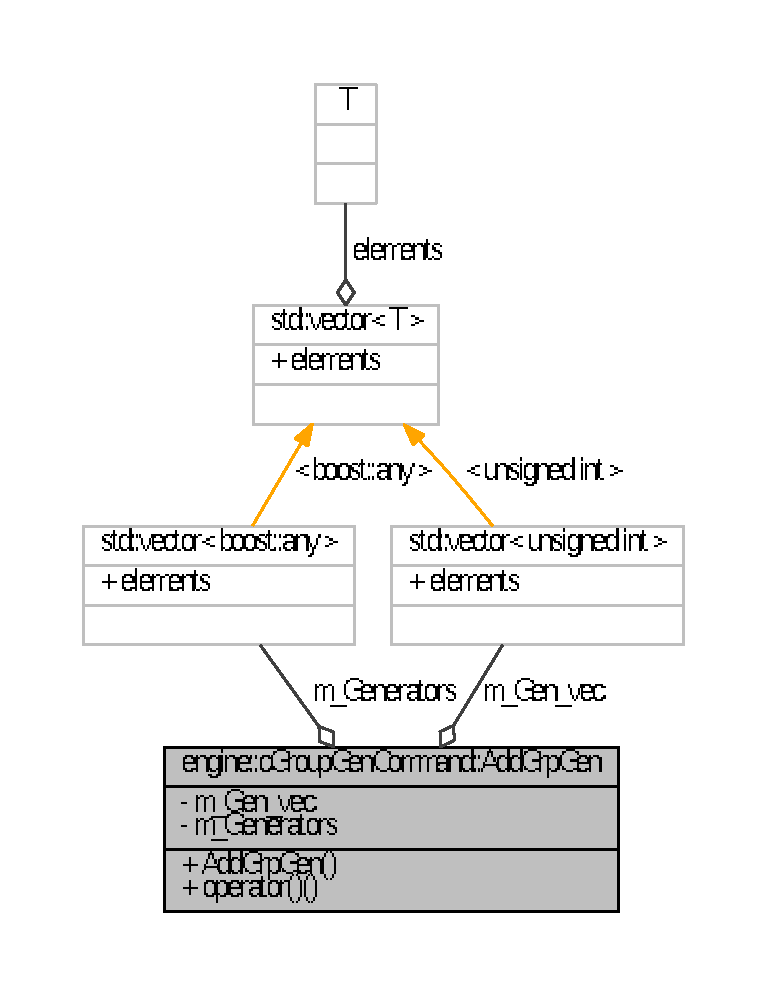
\includegraphics[width=350pt]{classengine_1_1cGroupGenCommand_1_1AddGrpGen__coll__graph}
\end{center}
\end{figure}
\subsection*{\-Public \-Member \-Functions}
\begin{DoxyCompactItemize}
\item 
\hypertarget{classengine_1_1cGroupGenCommand_1_1AddGrpGen_a274963aac553fde253b894ded1f01b11}{{\bfseries \-Add\-Grp\-Gen} (std\-::vector$<$ unsigned int $>$ $\ast$gen\-\_\-vec, std\-::vector$<$ boost\-::any $>$ $\ast$generators)}\label{classengine_1_1cGroupGenCommand_1_1AddGrpGen_a274963aac553fde253b894ded1f01b11}

\item 
\hypertarget{classengine_1_1cGroupGenCommand_1_1AddGrpGen_a686fa7657fd9467796a73cd84755d4b3}{void {\bfseries operator()} (char const \&i, qi\-::unused\-\_\-type, qi\-::unused\-\_\-type) const }\label{classengine_1_1cGroupGenCommand_1_1AddGrpGen_a686fa7657fd9467796a73cd84755d4b3}

\end{DoxyCompactItemize}
\subsection*{\-Private \-Attributes}
\begin{DoxyCompactItemize}
\item 
\hypertarget{classengine_1_1cGroupGenCommand_1_1AddGrpGen_a921873dbc006d113193b4c786d4c1902}{std\-::vector$<$ unsigned int $>$ $\ast$ {\bfseries m\-\_\-\-Gen\-\_\-vec}}\label{classengine_1_1cGroupGenCommand_1_1AddGrpGen_a921873dbc006d113193b4c786d4c1902}

\item 
\hypertarget{classengine_1_1cGroupGenCommand_1_1AddGrpGen_ab085284851fe15084450804f8b587414}{std\-::vector$<$ boost\-::any $>$ $\ast$ {\bfseries m\-\_\-\-Generators}}\label{classengine_1_1cGroupGenCommand_1_1AddGrpGen_ab085284851fe15084450804f8b587414}

\end{DoxyCompactItemize}


\-The documentation for this class was generated from the following file\-:\begin{DoxyCompactItemize}
\item 
groupgen\-\_\-command.\-h\end{DoxyCompactItemize}

\hypertarget{classengine_1_1cCommand}{\section{engine\-:\-:c\-Command Class Reference}
\label{classengine_1_1cCommand}\index{engine\-::c\-Command@{engine\-::c\-Command}}
}


Inheritance diagram for engine\-:\-:c\-Command\-:


Collaboration diagram for engine\-:\-:c\-Command\-:
\subsection*{Public Member Functions}
\begin{DoxyCompactItemize}
\item 
\hypertarget{classengine_1_1cCommand_a4c84c161b94f6ae36aec3661f951b54f}{virtual void {\bfseries Execute} ()=0}\label{classengine_1_1cCommand_a4c84c161b94f6ae36aec3661f951b54f}

\item 
virtual unsigned int \hyperlink{classengine_1_1cCommand_a8b5b45ad34530c454722a44e41ce9e78}{Estimate\-Run\-Time} (const \hyperlink{classengine_1_1cEstimator}{c\-Estimator} \&estimator) const =0
\end{DoxyCompactItemize}


\subsection{Member Function Documentation}
\hypertarget{classengine_1_1cCommand_a8b5b45ad34530c454722a44e41ce9e78}{\index{engine\-::c\-Command@{engine\-::c\-Command}!Estimate\-Run\-Time@{Estimate\-Run\-Time}}
\index{Estimate\-Run\-Time@{Estimate\-Run\-Time}!engine::cCommand@{engine\-::c\-Command}}
\subsubsection[{Estimate\-Run\-Time}]{\setlength{\rightskip}{0pt plus 5cm}virtual unsigned int engine\-::c\-Command\-::\-Estimate\-Run\-Time (
\begin{DoxyParamCaption}
\item[{const {\bf c\-Estimator} \&}]{estimator}
\end{DoxyParamCaption}
) const\hspace{0.3cm}{\ttfamily [pure virtual]}}}\label{classengine_1_1cCommand_a8b5b45ad34530c454722a44e41ce9e78}
uses the visitor based on \hyperlink{classengine_1_1cEstimator}{c\-Estimator} to return a rough estimation of the running time of a given command 

Implemented in \hyperlink{classengine_1_1cGetElemCommand_ad84c73fe5b4db65679f28c427d201434}{engine\-::c\-Get\-Elem\-Command}, \hyperlink{classengine_1_1cGetCenterCommand_ab00fa221228c2550e8f664c6d887e1e0}{engine\-::c\-Get\-Center\-Command}, \hyperlink{classengine_1_1cGetCGraphCommand_a0a3d07c4f82227b7f0ffbcf01f7fcec2}{engine\-::c\-Get\-C\-Graph\-Command}, and \hyperlink{classengine_1_1cGetRelCommand_ad6aa9cb526ae1b73237edaad02d081ec}{engine\-::c\-Get\-Rel\-Command}.



The documentation for this class was generated from the following file\-:\begin{DoxyCompactItemize}
\item 
command.\-h\end{DoxyCompactItemize}

\hypertarget{classengine_1_1cCommandCreator}{
\section{engine\-:\-:c\-Command\-Creator$<$ \-C\-R\-E\-A\-T\-O\-R $>$ \-Class \-Template \-Reference}
\label{classengine_1_1cCommandCreator}\index{engine\-::c\-Command\-Creator$<$ C\-R\-E\-A\-T\-O\-R $>$@{engine\-::c\-Command\-Creator$<$ C\-R\-E\-A\-T\-O\-R $>$}}
}
\subsection*{\-Static \-Public \-Member \-Functions}
\begin{DoxyCompactItemize}
\item 
\hypertarget{classengine_1_1cCommandCreator_a37ff251d6e86ded9b9893cf66a635cd2}{
static \hyperlink{classengine_1_1cCommand}{c\-Command} $\ast$ {\bfseries \-Get\-Command} (\-C\-O\-M\-M\-A\-N\-D\-\_\-\-T\-Y\-P\-E command, const std\-::string \&param, \hyperlink{classengine_1_1cResult}{c\-Result} $\ast$result)}
\label{classengine_1_1cCommandCreator_a37ff251d6e86ded9b9893cf66a635cd2}

\end{DoxyCompactItemize}
\subsubsection*{template$<$typename C\-R\-E\-A\-T\-O\-R$>$ class engine\-::c\-Command\-Creator$<$ C\-R\-E\-A\-T\-O\-R $>$}



\-The documentation for this class was generated from the following file\-:\begin{DoxyCompactItemize}
\item 
command\-\_\-creator.\-h\end{DoxyCompactItemize}

\hypertarget{classengine_1_1cCommandQueue}{\section{engine\-:\-:c\-Command\-Queue \-Class \-Reference}
\label{classengine_1_1cCommandQueue}\index{engine\-::c\-Command\-Queue@{engine\-::c\-Command\-Queue}}
}


{\ttfamily \#include $<$command\-\_\-queue.\-h$>$}



\-Collaboration diagram for engine\-:\-:c\-Command\-Queue\-:\nopagebreak
\begin{figure}[H]
\begin{center}
\leavevmode
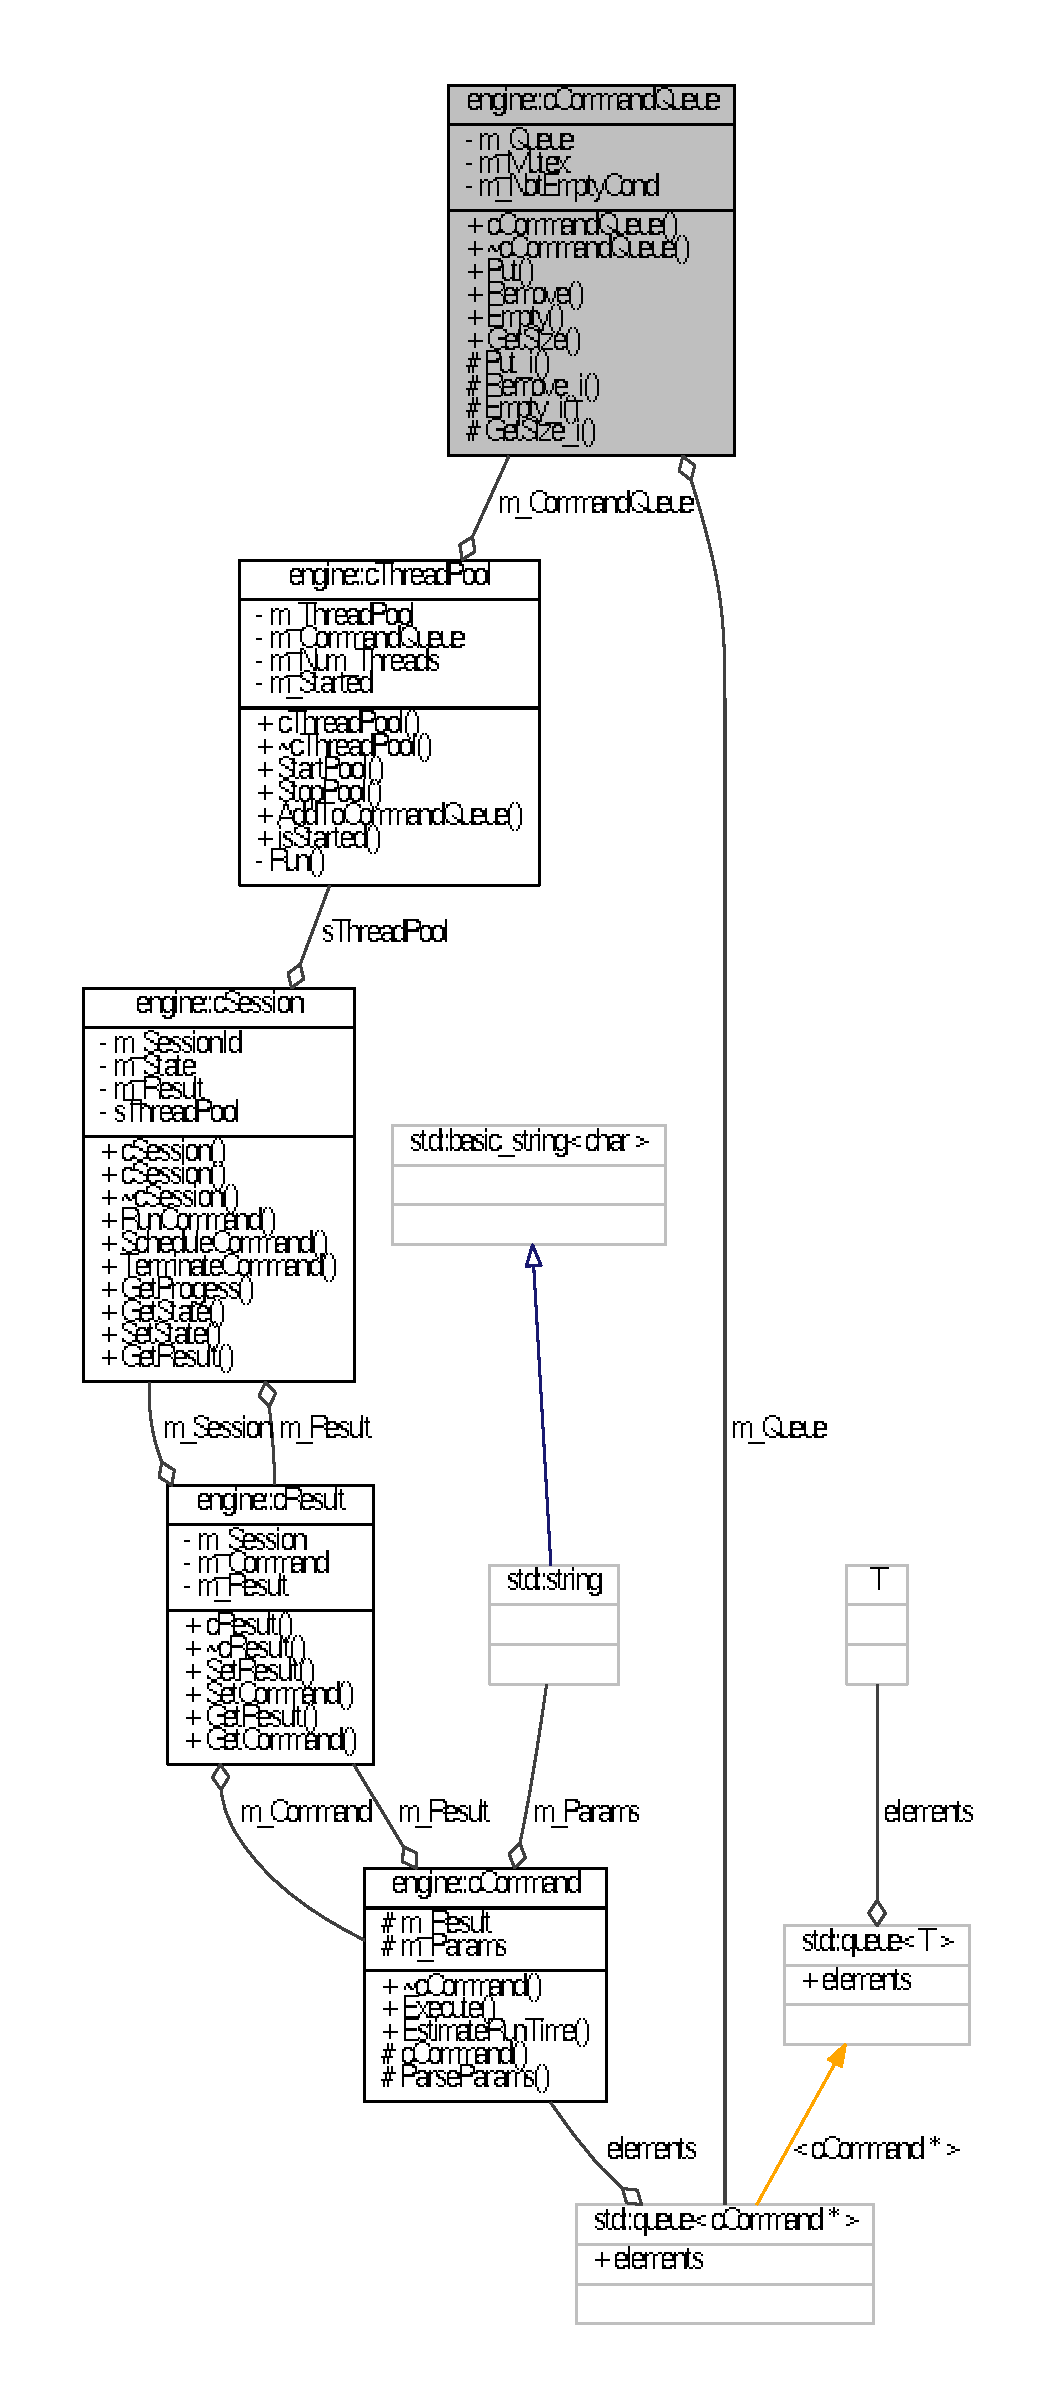
\includegraphics[height=550pt]{classengine_1_1cCommandQueue__coll__graph}
\end{center}
\end{figure}
\subsection*{\-Public \-Member \-Functions}
\begin{DoxyCompactItemize}
\item 
\hypertarget{classengine_1_1cCommandQueue_a1d60f01d5e9bd4d17c892257e20b2b89}{void {\bfseries \-Put} (\hyperlink{classengine_1_1cCommand}{c\-Command} $\ast$command)}\label{classengine_1_1cCommandQueue_a1d60f01d5e9bd4d17c892257e20b2b89}

\item 
\hypertarget{classengine_1_1cCommandQueue_a7979f6e2a55a331083c879f4265895f5}{\hyperlink{classengine_1_1cCommand}{c\-Command} $\ast$ {\bfseries \-Remove} ()}\label{classengine_1_1cCommandQueue_a7979f6e2a55a331083c879f4265895f5}

\item 
\hypertarget{classengine_1_1cCommandQueue_a727d36f68de37caba84869e3f973ccbc}{bool {\bfseries \-Empty} ()}\label{classengine_1_1cCommandQueue_a727d36f68de37caba84869e3f973ccbc}

\item 
\hypertarget{classengine_1_1cCommandQueue_af6b95fb876418671d6285ee368abca25}{std\-::size\-\_\-t {\bfseries \-Get\-Size} ()}\label{classengine_1_1cCommandQueue_af6b95fb876418671d6285ee368abca25}

\end{DoxyCompactItemize}
\subsection*{\-Protected \-Member \-Functions}
\begin{DoxyCompactItemize}
\item 
\hypertarget{classengine_1_1cCommandQueue_a3e66c5c4390594c00276229ddf2d3e39}{void {\bfseries \-Put\-\_\-i} (\hyperlink{classengine_1_1cCommand}{c\-Command} $\ast$command)}\label{classengine_1_1cCommandQueue_a3e66c5c4390594c00276229ddf2d3e39}

\item 
\hypertarget{classengine_1_1cCommandQueue_acaee2664e59c4e91aeeac18066df9716}{\hyperlink{classengine_1_1cCommand}{c\-Command} $\ast$ {\bfseries \-Remove\-\_\-i} ()}\label{classengine_1_1cCommandQueue_acaee2664e59c4e91aeeac18066df9716}

\item 
\hypertarget{classengine_1_1cCommandQueue_a7c8a6bd8dae5c050634cededcb77ef4d}{bool {\bfseries \-Empty\-\_\-i} () const }\label{classengine_1_1cCommandQueue_a7c8a6bd8dae5c050634cededcb77ef4d}

\item 
\hypertarget{classengine_1_1cCommandQueue_a2b729f6d9866c6e9b50e142f7e475b05}{std\-::size\-\_\-t {\bfseries \-Get\-Size\-\_\-i} () const }\label{classengine_1_1cCommandQueue_a2b729f6d9866c6e9b50e142f7e475b05}

\end{DoxyCompactItemize}
\subsection*{\-Private \-Attributes}
\begin{DoxyCompactItemize}
\item 
\hypertarget{classengine_1_1cCommandQueue_acab17ed41f5114d5baaf14a6f8641e96}{std\-::queue$<$ \hyperlink{classengine_1_1cCommand}{c\-Command} $\ast$ $>$ {\bfseries m\-\_\-\-Queue}}\label{classengine_1_1cCommandQueue_acab17ed41f5114d5baaf14a6f8641e96}

\item 
\hypertarget{classengine_1_1cCommandQueue_a3382d012fe90188199630bef438d7901}{boost\-::mutex {\bfseries m\-\_\-\-Mutex}}\label{classengine_1_1cCommandQueue_a3382d012fe90188199630bef438d7901}

\item 
\hypertarget{classengine_1_1cCommandQueue_a7edc3ed909364aca4956ff6b8d95b912}{boost\-::condition\-\_\-variable {\bfseries m\-\_\-\-Not\-Empty\-Cond}}\label{classengine_1_1cCommandQueue_a7edc3ed909364aca4956ff6b8d95b912}

\end{DoxyCompactItemize}


\subsection{\-Detailed \-Description}
thread safe class that implements a commands queue used to keep the command until the worker threads from the pool executes them (half sync half async pattern) used design patterns\-: thread safe interface, monitor object, half-\/sync, half-\/async 

\-The documentation for this class was generated from the following files\-:\begin{DoxyCompactItemize}
\item 
command\-\_\-queue.\-h\item 
command\-\_\-queue.\-cpp\end{DoxyCompactItemize}

\hypertarget{classengine_1_1cCreator}{\section{engine\-:\-:c\-Creator \-Class \-Reference}
\label{classengine_1_1cCreator}\index{engine\-::c\-Creator@{engine\-::c\-Creator}}
}


{\ttfamily \#include $<$command\-\_\-creator.\-h$>$}

\subsection*{\-Static \-Public \-Member \-Functions}
\begin{DoxyCompactItemize}
\item 
\hypertarget{classengine_1_1cCreator_a67c7b575c0a32a48bb2428d263ccd3e0}{static \hyperlink{classengine_1_1cCommand}{c\-Command} $\ast$ {\bfseries \-Get\-Command} (\-C\-O\-M\-M\-A\-N\-D\-\_\-\-T\-Y\-P\-E command, const std\-::string \&param, \hyperlink{classengine_1_1cResult}{c\-Result} $\ast$result)}\label{classengine_1_1cCreator_a67c7b575c0a32a48bb2428d263ccd3e0}

\end{DoxyCompactItemize}


\subsection{\-Detailed \-Description}
implements the default command creation strategy 

\-The documentation for this class was generated from the following file\-:\begin{DoxyCompactItemize}
\item 
command\-\_\-creator.\-h\end{DoxyCompactItemize}

\hypertarget{classengine_1_1cEstimator}{\section{engine\-:\-:c\-Estimator \-Class \-Reference}
\label{classengine_1_1cEstimator}\index{engine\-::c\-Estimator@{engine\-::c\-Estimator}}
}


{\ttfamily \#include $<$estimate.\-h$>$}

\subsection*{\-Public \-Member \-Functions}
\begin{DoxyCompactItemize}
\item 
\hypertarget{classengine_1_1cEstimator_a6d2c3458e2ce412c10a355d651d9b98f}{virtual std\-::size\-\_\-t {\bfseries \-Estimate} (const \hyperlink{classengine_1_1cGetElemCommand}{c\-Get\-Elem\-Command} \&getelem\-\_\-command) const }\label{classengine_1_1cEstimator_a6d2c3458e2ce412c10a355d651d9b98f}

\item 
\hypertarget{classengine_1_1cEstimator_af6bcdcbb321c9d700571cf6fa1c06925}{virtual std\-::size\-\_\-t {\bfseries \-Estimate} (const \hyperlink{classengine_1_1cGetCenterCommand}{c\-Get\-Center\-Command} \&getcenter\-\_\-command) const }\label{classengine_1_1cEstimator_af6bcdcbb321c9d700571cf6fa1c06925}

\item 
\hypertarget{classengine_1_1cEstimator_add065c4c480b539c47b53195d6426764}{virtual std\-::size\-\_\-t {\bfseries \-Estimate} (const \hyperlink{classengine_1_1cGetCGraphCommand}{c\-Get\-C\-Graph\-Command} \&getcgraph\-\_\-command) const }\label{classengine_1_1cEstimator_add065c4c480b539c47b53195d6426764}

\end{DoxyCompactItemize}


\subsection{\-Detailed \-Description}
base class for command estimators should be used as a visitor in the command class(\-Estimate(c\-Estimator\&)) 

\-The documentation for this class was generated from the following files\-:\begin{DoxyCompactItemize}
\item 
estimate.\-h\item 
estimate.\-cpp\end{DoxyCompactItemize}

\hypertarget{classengine_1_1cGetCenterCommand}{\section{engine\-:\-:c\-Get\-Center\-Command \-Class \-Reference}
\label{classengine_1_1cGetCenterCommand}\index{engine\-::c\-Get\-Center\-Command@{engine\-::c\-Get\-Center\-Command}}
}


{\ttfamily \#include $<$getcenter\-\_\-command.\-h$>$}



\-Inheritance diagram for engine\-:\-:c\-Get\-Center\-Command\-:
\nopagebreak
\begin{figure}[H]
\begin{center}
\leavevmode
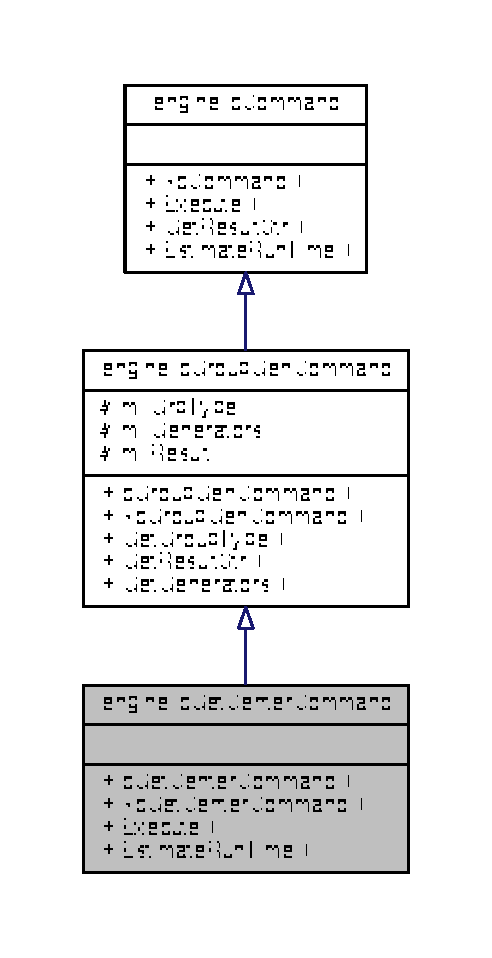
\includegraphics[width=236pt]{classengine_1_1cGetCenterCommand__inherit__graph}
\end{center}
\end{figure}


\-Collaboration diagram for engine\-:\-:c\-Get\-Center\-Command\-:
\nopagebreak
\begin{figure}[H]
\begin{center}
\leavevmode
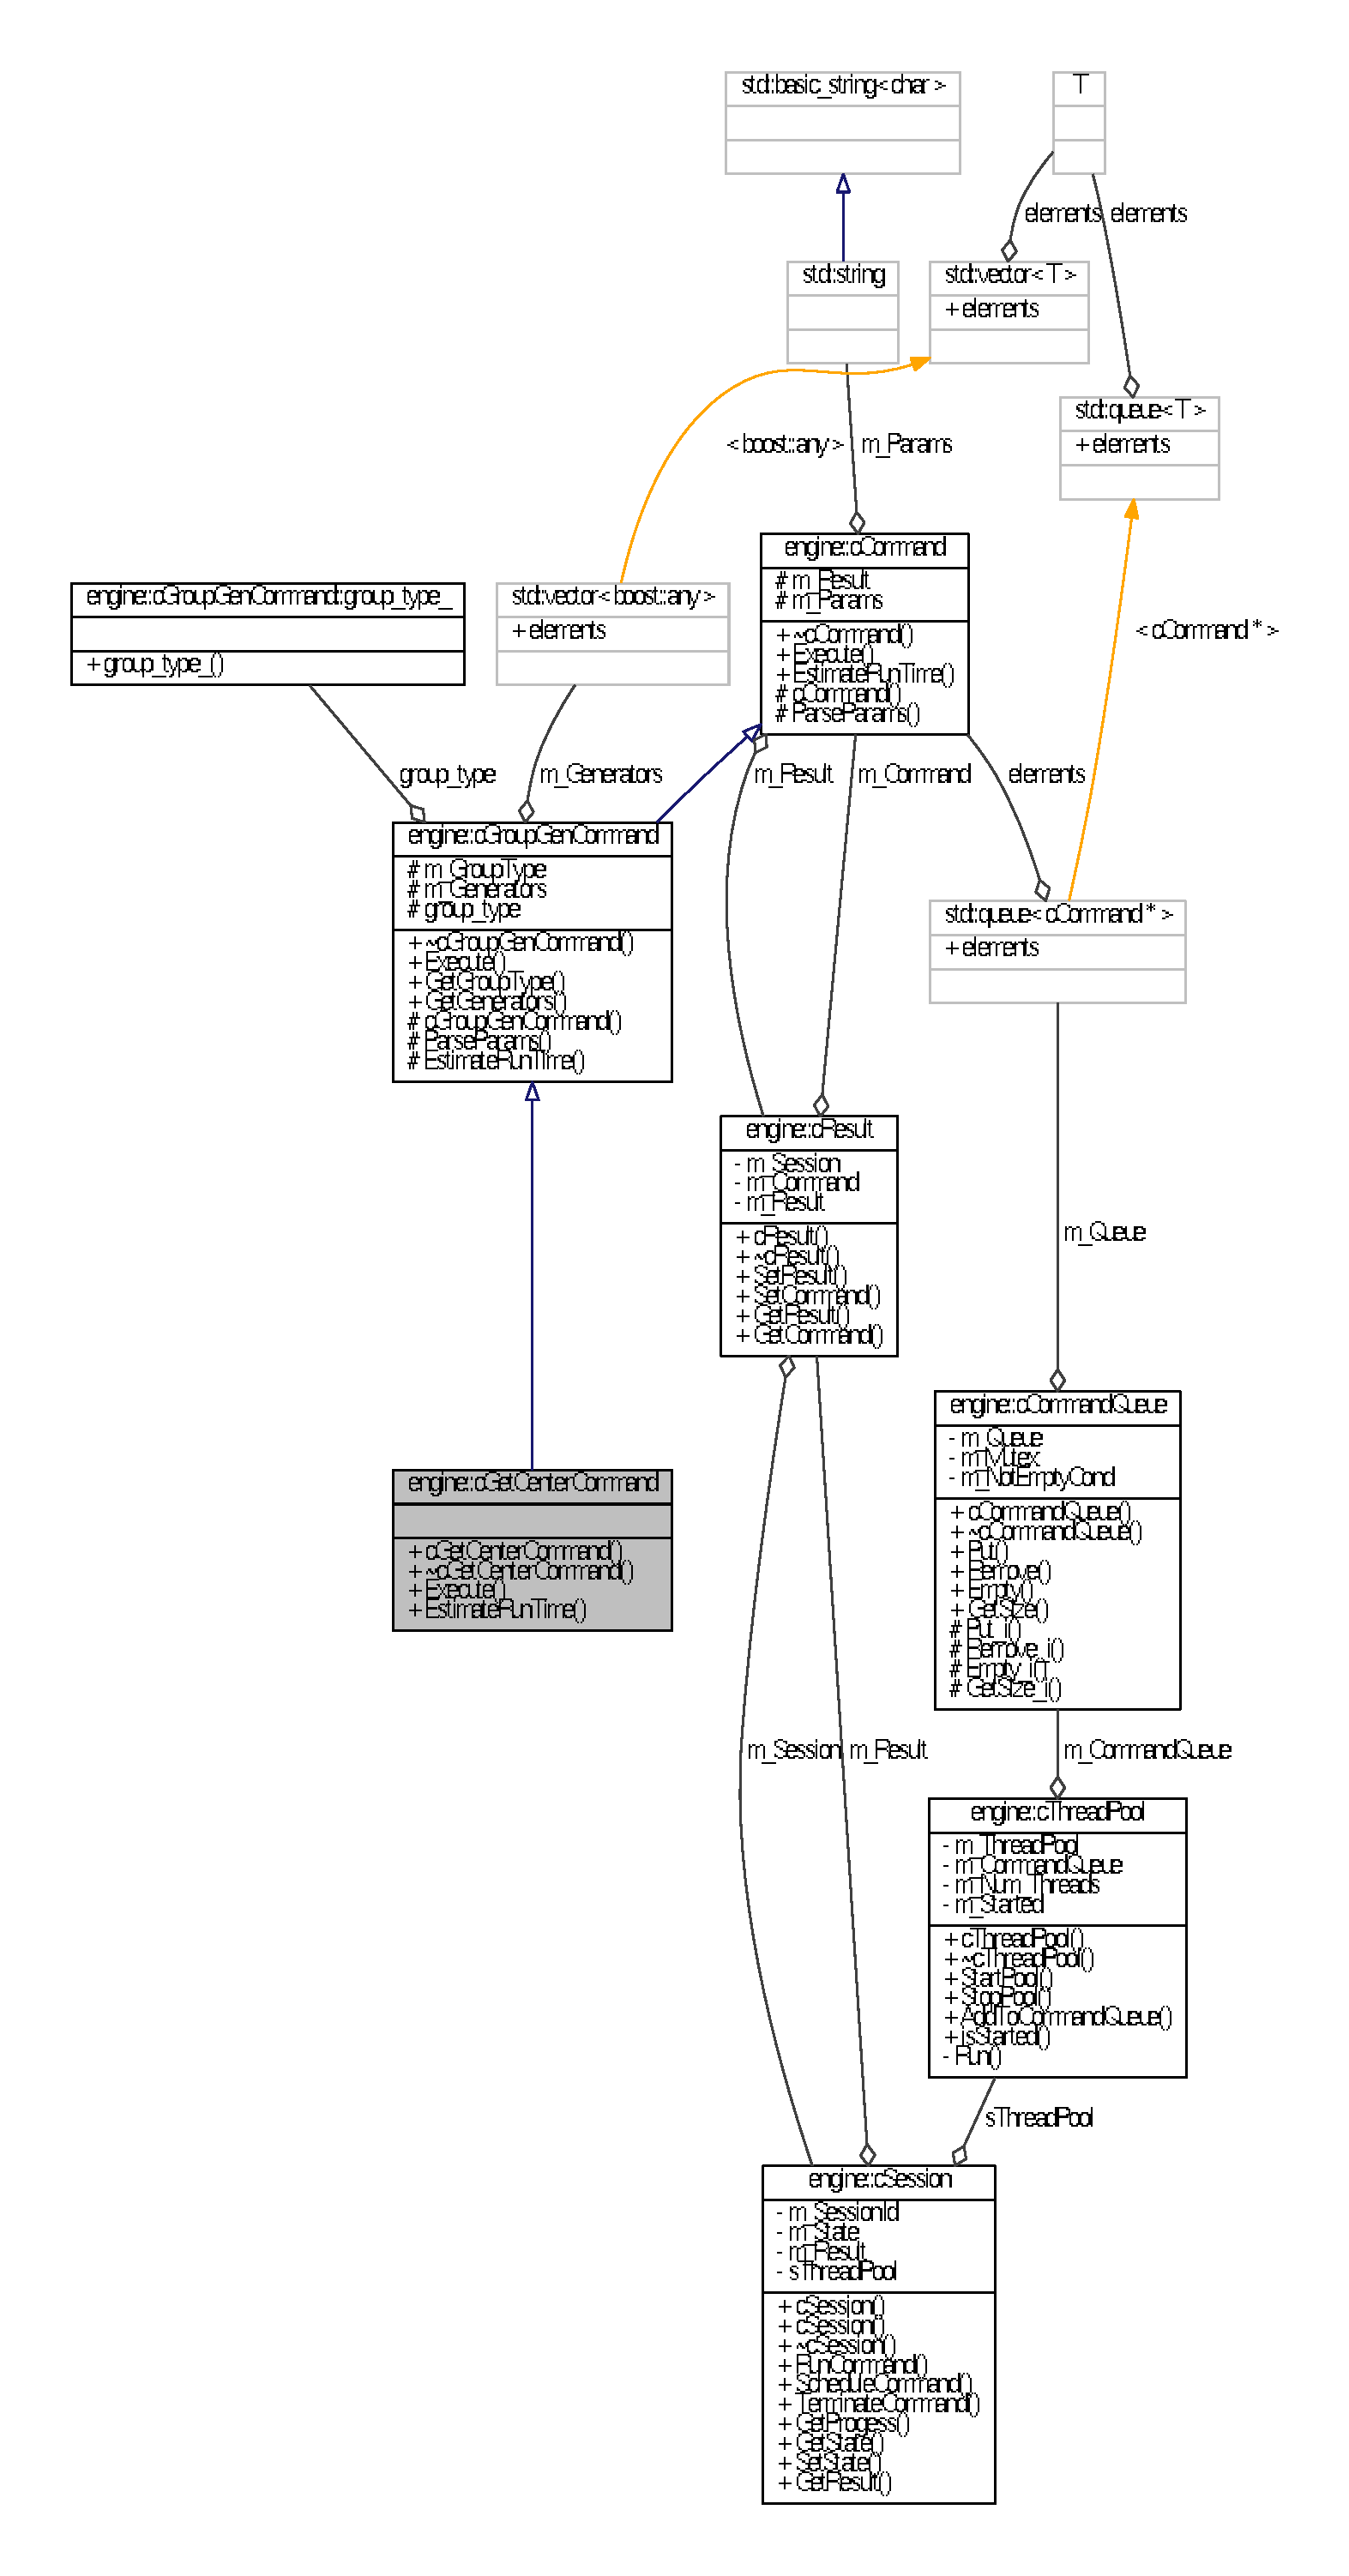
\includegraphics[height=550pt]{classengine_1_1cGetCenterCommand__coll__graph}
\end{center}
\end{figure}
\subsection*{\-Public \-Member \-Functions}
\begin{DoxyCompactItemize}
\item 
\hypertarget{classengine_1_1cGetCenterCommand_ae215414c205174cc048d63174f19fd3a}{{\bfseries c\-Get\-Center\-Command} (const std\-::string \&params, \hyperlink{classengine_1_1cResult}{c\-Result} $\ast$result)}\label{classengine_1_1cGetCenterCommand_ae215414c205174cc048d63174f19fd3a}

\item 
\hypertarget{classengine_1_1cGetCenterCommand_a7d2754e5ade6a96e6043547a7f2b1a03}{void {\bfseries \-Execute} ()}\label{classengine_1_1cGetCenterCommand_a7d2754e5ade6a96e6043547a7f2b1a03}

\item 
unsigned int \hyperlink{classengine_1_1cGetCenterCommand_ab00fa221228c2550e8f664c6d887e1e0}{\-Estimate\-Run\-Time} (const \hyperlink{classengine_1_1cEstimator}{c\-Estimator} \&estimator) const 
\end{DoxyCompactItemize}


\subsection{\-Detailed \-Description}
command that obtains the center of the group 

\subsection{\-Member \-Function \-Documentation}
\hypertarget{classengine_1_1cGetCenterCommand_ab00fa221228c2550e8f664c6d887e1e0}{\index{engine\-::c\-Get\-Center\-Command@{engine\-::c\-Get\-Center\-Command}!\-Estimate\-Run\-Time@{\-Estimate\-Run\-Time}}
\index{\-Estimate\-Run\-Time@{\-Estimate\-Run\-Time}!engine::cGetCenterCommand@{engine\-::c\-Get\-Center\-Command}}
\subsubsection[{\-Estimate\-Run\-Time}]{\setlength{\rightskip}{0pt plus 5cm}unsigned int {\bf engine\-::c\-Get\-Center\-Command\-::\-Estimate\-Run\-Time} (
\begin{DoxyParamCaption}
\item[{const {\bf c\-Estimator} \&}]{estimator}
\end{DoxyParamCaption}
) const\hspace{0.3cm}{\ttfamily  \mbox{[}virtual\mbox{]}}}}\label{classengine_1_1cGetCenterCommand_ab00fa221228c2550e8f664c6d887e1e0}
uses the visitor based on \hyperlink{classengine_1_1cEstimator}{c\-Estimator} to return a rough estimation of the running time of a given command 

\-Implements \hyperlink{classengine_1_1cGroupGenCommand_aba96a75b873e66979b653f4e27540f3f}{engine\-::c\-Group\-Gen\-Command}.



\-The documentation for this class was generated from the following files\-:\begin{DoxyCompactItemize}
\item 
getcenter\-\_\-command.\-h\item 
getcenter\-\_\-command.\-cpp\end{DoxyCompactItemize}

\hypertarget{classengine_1_1cGetCGraphCommand}{\section{engine\-:\-:c\-Get\-C\-Graph\-Command \-Class \-Reference}
\label{classengine_1_1cGetCGraphCommand}\index{engine\-::c\-Get\-C\-Graph\-Command@{engine\-::c\-Get\-C\-Graph\-Command}}
}


{\ttfamily \#include $<$getcgraph\-\_\-command.\-h$>$}



\-Inheritance diagram for engine\-:\-:c\-Get\-C\-Graph\-Command\-:
\nopagebreak
\begin{figure}[H]
\begin{center}
\leavevmode
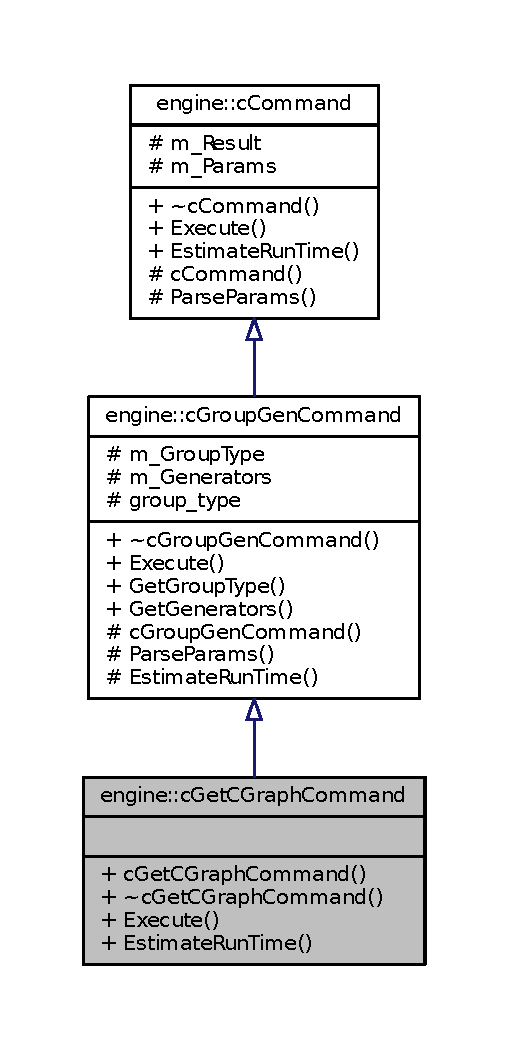
\includegraphics[width=240pt]{classengine_1_1cGetCGraphCommand__inherit__graph}
\end{center}
\end{figure}


\-Collaboration diagram for engine\-:\-:c\-Get\-C\-Graph\-Command\-:
\nopagebreak
\begin{figure}[H]
\begin{center}
\leavevmode
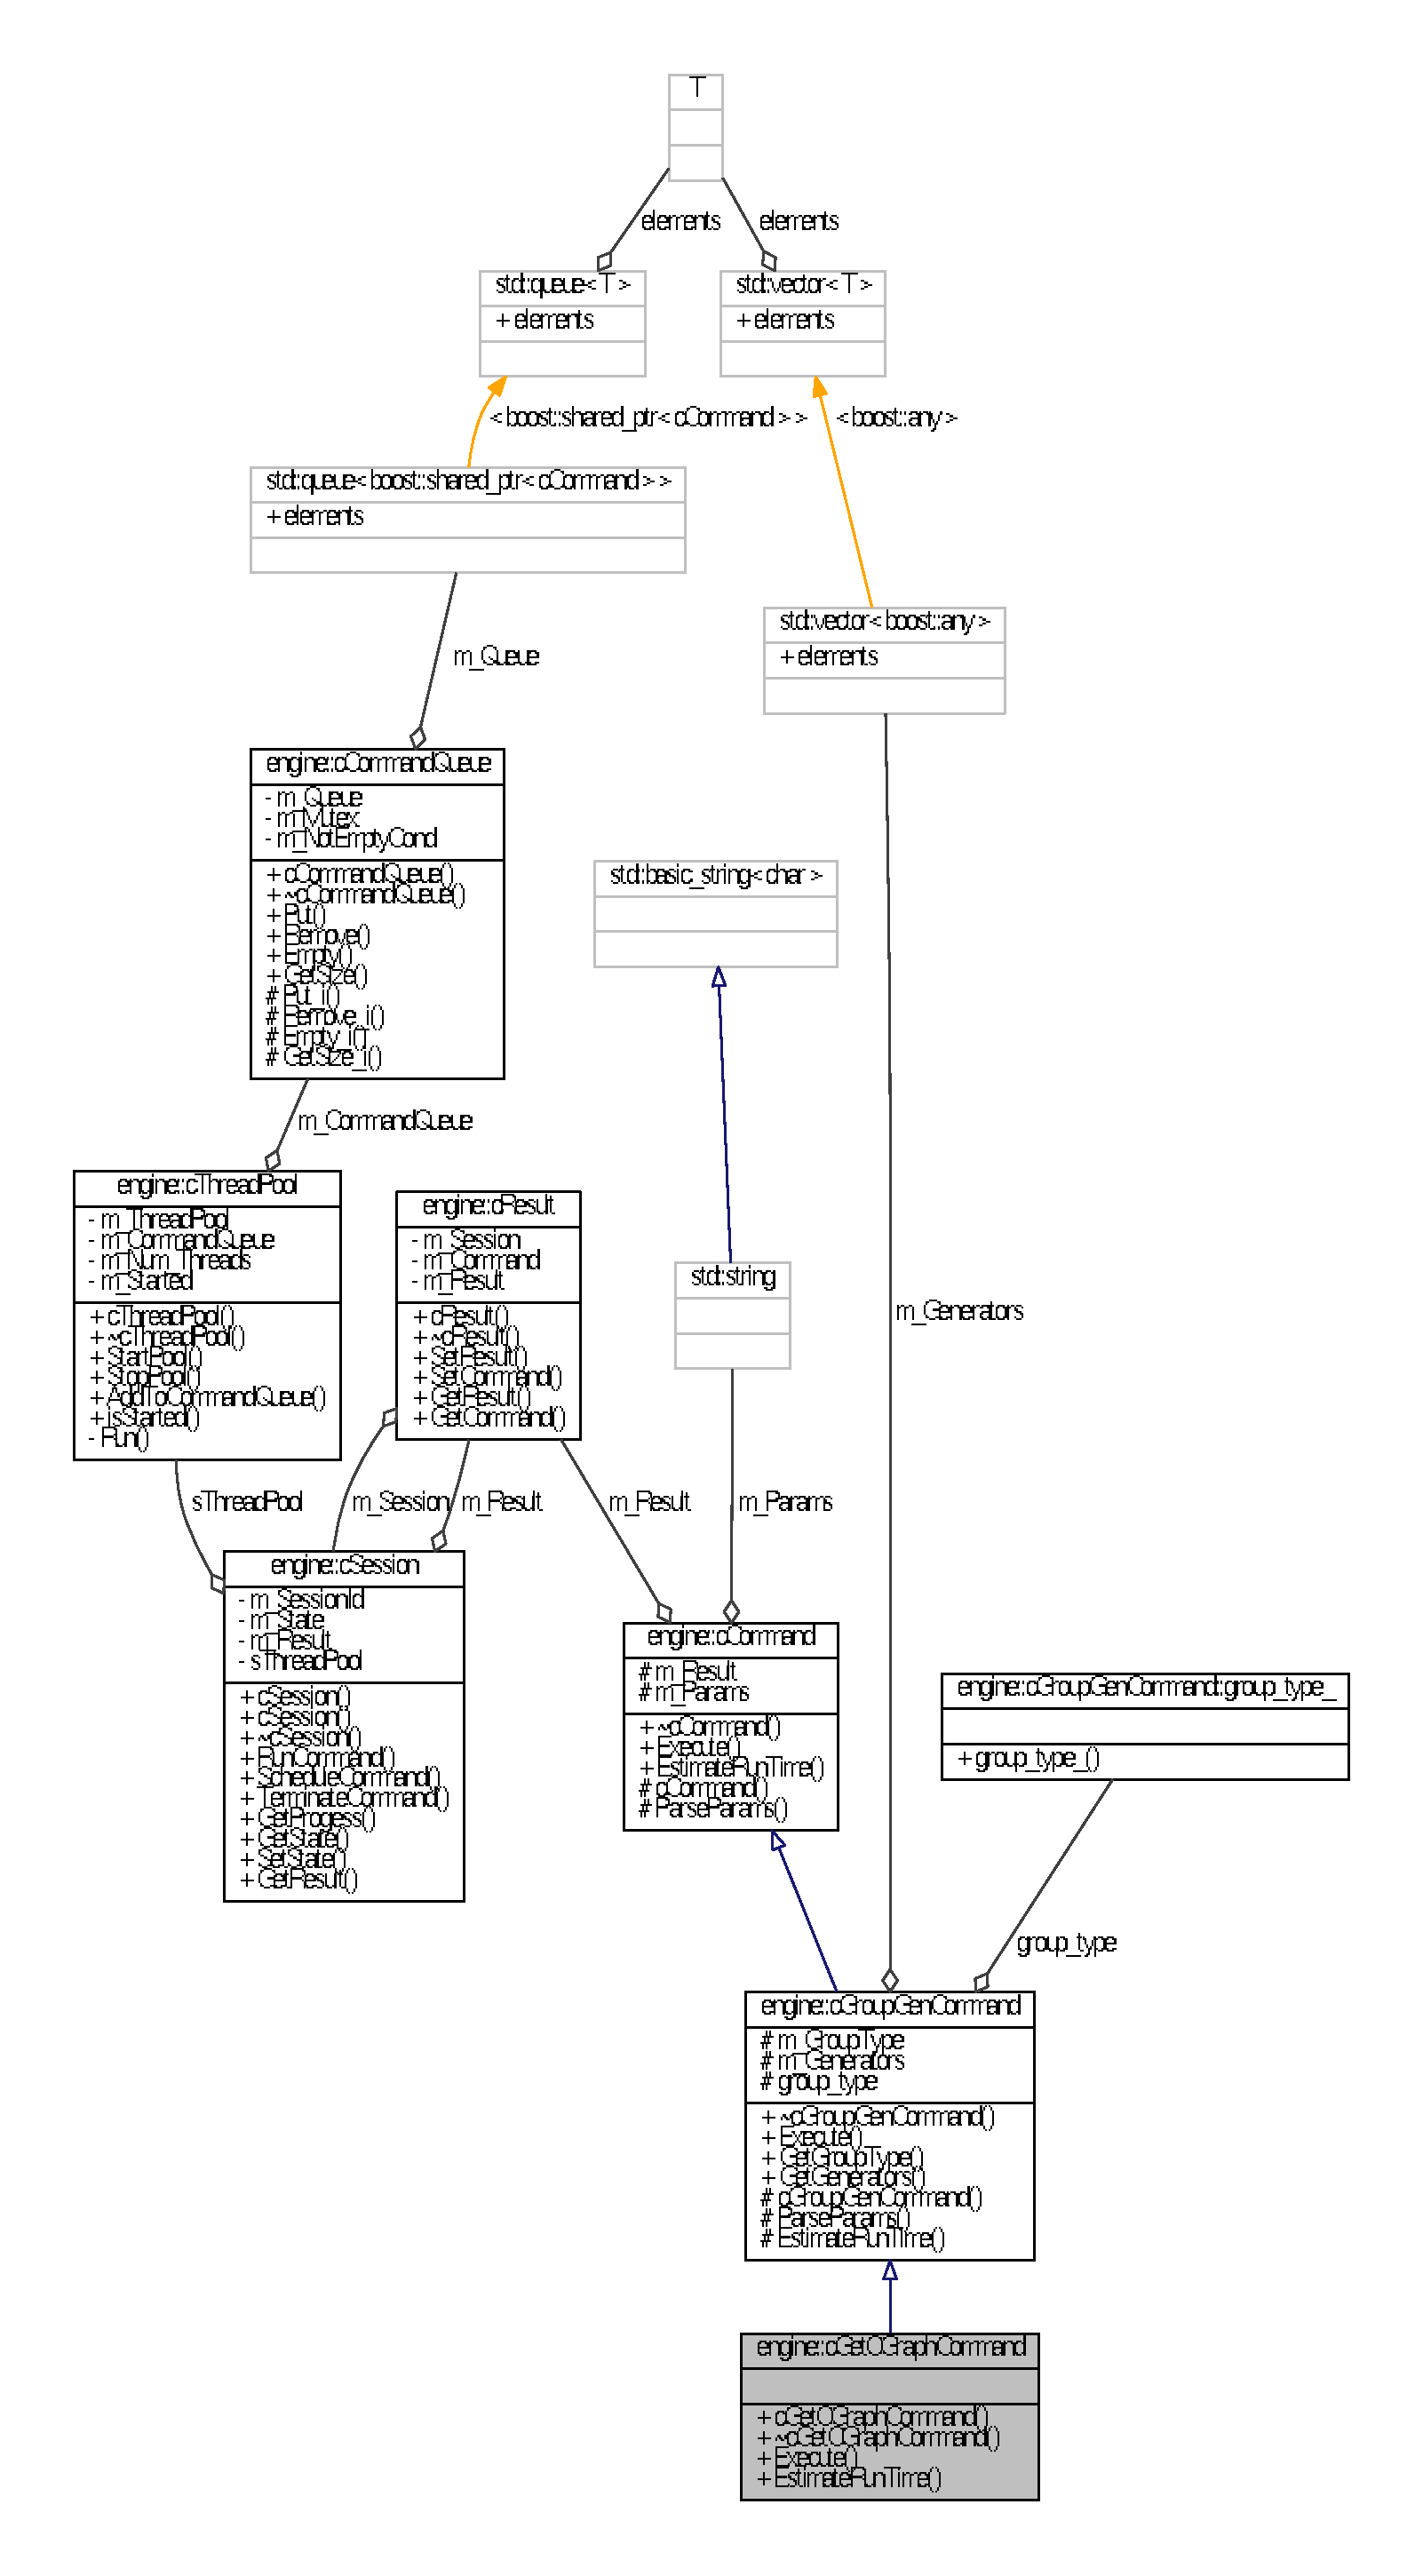
\includegraphics[height=550pt]{classengine_1_1cGetCGraphCommand__coll__graph}
\end{center}
\end{figure}
\subsection*{\-Public \-Member \-Functions}
\begin{DoxyCompactItemize}
\item 
\hypertarget{classengine_1_1cGetCGraphCommand_aaf87f44392cf780bd4308e8d6dc3139d}{{\bfseries c\-Get\-C\-Graph\-Command} (const std\-::string \&params, \hyperlink{classengine_1_1cResult}{c\-Result} $\ast$result)}\label{classengine_1_1cGetCGraphCommand_aaf87f44392cf780bd4308e8d6dc3139d}

\item 
\hypertarget{classengine_1_1cGetCGraphCommand_a94b83bc4b3103138411ec5bf1ccca84c}{void {\bfseries \-Execute} ()}\label{classengine_1_1cGetCGraphCommand_a94b83bc4b3103138411ec5bf1ccca84c}

\item 
unsigned int \hyperlink{classengine_1_1cGetCGraphCommand_a0a3d07c4f82227b7f0ffbcf01f7fcec2}{\-Estimate\-Run\-Time} (const \hyperlink{classengine_1_1cEstimator}{c\-Estimator} \&estimator) const 
\end{DoxyCompactItemize}


\subsection{\-Detailed \-Description}
command that obtains \-Cayley graph of the group 

\subsection{\-Member \-Function \-Documentation}
\hypertarget{classengine_1_1cGetCGraphCommand_a0a3d07c4f82227b7f0ffbcf01f7fcec2}{\index{engine\-::c\-Get\-C\-Graph\-Command@{engine\-::c\-Get\-C\-Graph\-Command}!\-Estimate\-Run\-Time@{\-Estimate\-Run\-Time}}
\index{\-Estimate\-Run\-Time@{\-Estimate\-Run\-Time}!engine::cGetCGraphCommand@{engine\-::c\-Get\-C\-Graph\-Command}}
\subsubsection[{\-Estimate\-Run\-Time}]{\setlength{\rightskip}{0pt plus 5cm}unsigned int {\bf engine\-::c\-Get\-C\-Graph\-Command\-::\-Estimate\-Run\-Time} (
\begin{DoxyParamCaption}
\item[{const {\bf c\-Estimator} \&}]{estimator}
\end{DoxyParamCaption}
) const\hspace{0.3cm}{\ttfamily  \mbox{[}virtual\mbox{]}}}}\label{classengine_1_1cGetCGraphCommand_a0a3d07c4f82227b7f0ffbcf01f7fcec2}
uses the visitor based on \hyperlink{classengine_1_1cEstimator}{c\-Estimator} to return a rough estimation of the running time of a given command 

\-Implements \hyperlink{classengine_1_1cGroupGenCommand_aba96a75b873e66979b653f4e27540f3f}{engine\-::c\-Group\-Gen\-Command}.



\-The documentation for this class was generated from the following files\-:\begin{DoxyCompactItemize}
\item 
getcgraph\-\_\-command.\-h\item 
getcgraph\-\_\-command.\-cpp\end{DoxyCompactItemize}

\hypertarget{classengine_1_1cGetElemCommand}{
\section{engine\-:\-:c\-Get\-Elem\-Command \-Class \-Reference}
\label{classengine_1_1cGetElemCommand}\index{engine\-::c\-Get\-Elem\-Command@{engine\-::c\-Get\-Elem\-Command}}
}


\-Inheritance diagram for engine\-:\-:c\-Get\-Elem\-Command\-:\nopagebreak
\begin{figure}[H]
\begin{center}
\leavevmode
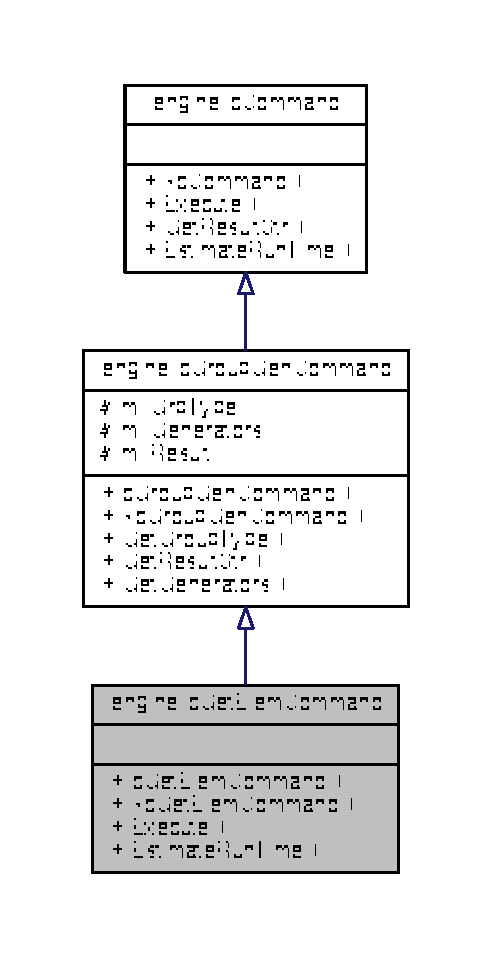
\includegraphics[width=238pt]{classengine_1_1cGetElemCommand__inherit__graph}
\end{center}
\end{figure}


\-Collaboration diagram for engine\-:\-:c\-Get\-Elem\-Command\-:\nopagebreak
\begin{figure}[H]
\begin{center}
\leavevmode
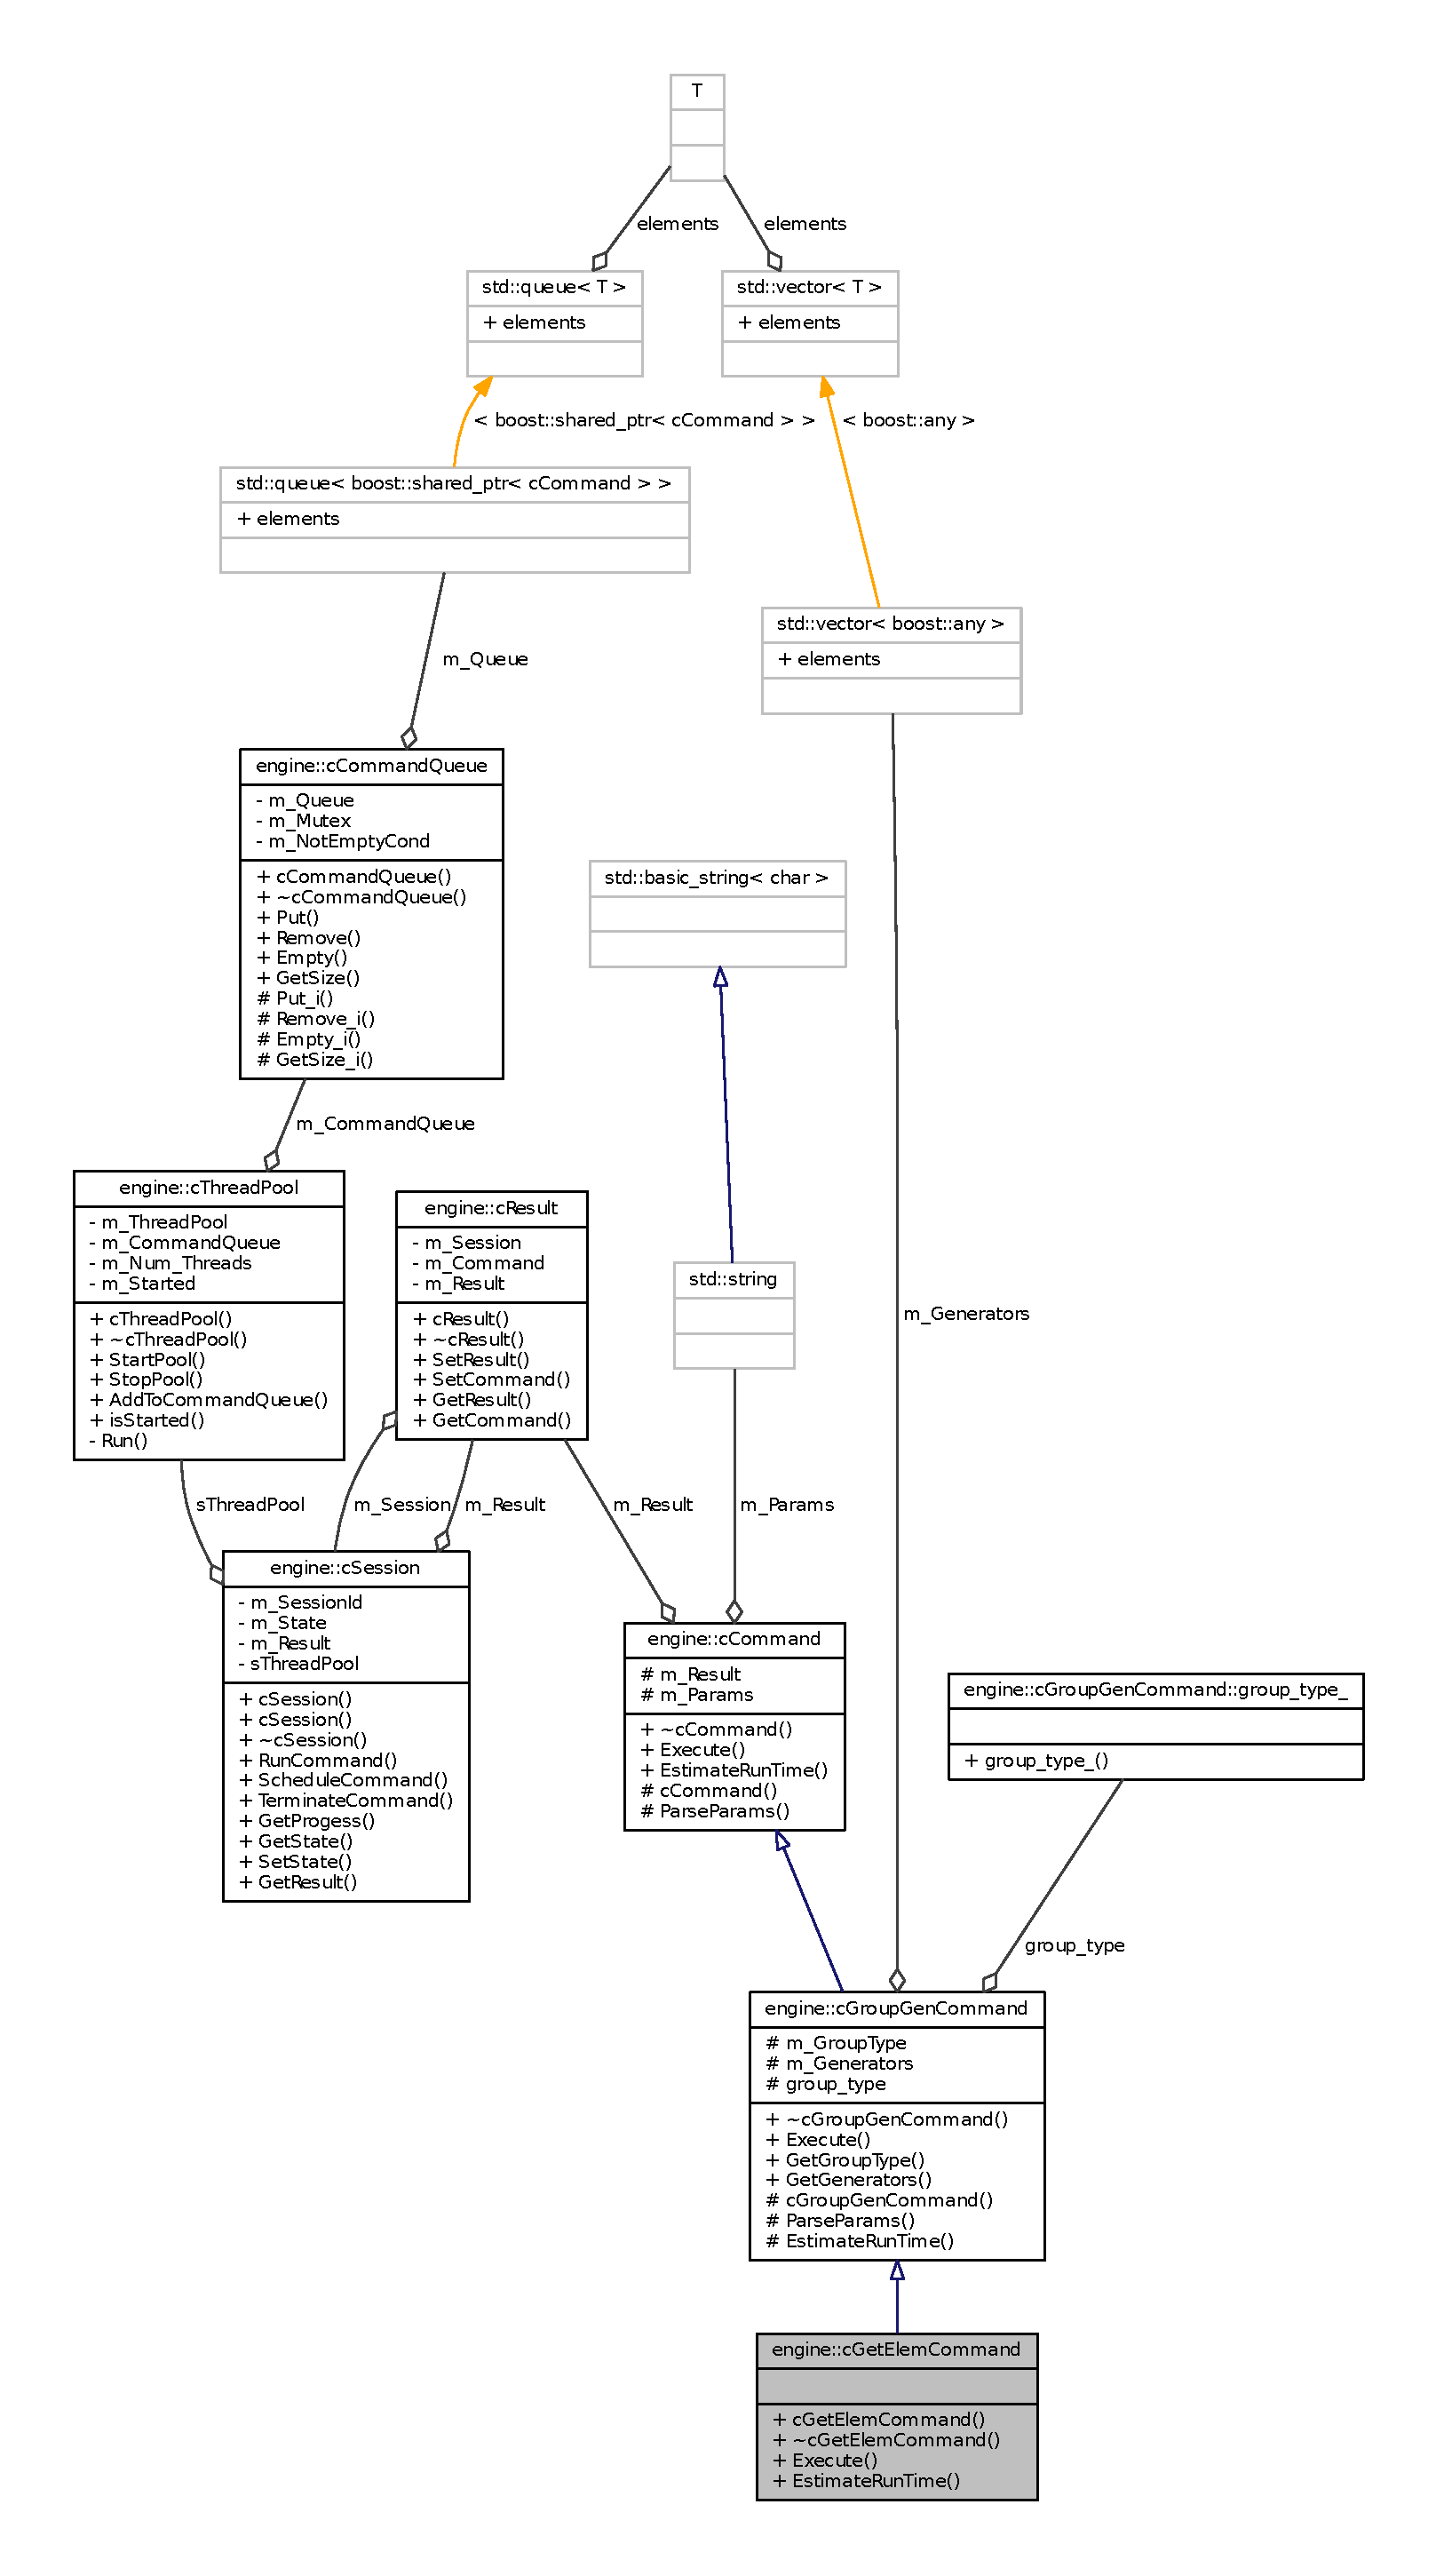
\includegraphics[height=550pt]{classengine_1_1cGetElemCommand__coll__graph}
\end{center}
\end{figure}
\subsection*{\-Public \-Member \-Functions}
\begin{DoxyCompactItemize}
\item 
\hypertarget{classengine_1_1cGetElemCommand_ae65189d2ef82b1ca49295268846b1dd6}{
{\bfseries c\-Get\-Elem\-Command} (const std\-::string \&params, \hyperlink{classengine_1_1cResult}{c\-Result} $\ast$result)}
\label{classengine_1_1cGetElemCommand_ae65189d2ef82b1ca49295268846b1dd6}

\item 
\hypertarget{classengine_1_1cGetElemCommand_a16a627c20d55b3f2538bab7f63a04a04}{
void {\bfseries \-Execute} ()}
\label{classengine_1_1cGetElemCommand_a16a627c20d55b3f2538bab7f63a04a04}

\item 
\hypertarget{classengine_1_1cGetElemCommand_ad84c73fe5b4db65679f28c427d201434}{
unsigned int {\bfseries \-Estimate\-Run\-Time} (const \hyperlink{classengine_1_1cEstimator}{c\-Estimator} \&estimator) const }
\label{classengine_1_1cGetElemCommand_ad84c73fe5b4db65679f28c427d201434}

\end{DoxyCompactItemize}


\-The documentation for this class was generated from the following files\-:\begin{DoxyCompactItemize}
\item 
getelem\-\_\-command.\-h\item 
getelem\-\_\-command.\-cpp\end{DoxyCompactItemize}

\hypertarget{classcGroupFactory}{\section{c\-Group\-Factory Class Reference}
\label{classcGroupFactory}\index{c\-Group\-Factory@{c\-Group\-Factory}}
}


{\ttfamily \#include $<$group\-\_\-factory.\-h$>$}



Collaboration diagram for c\-Group\-Factory\-:
\nopagebreak
\begin{figure}[H]
\begin{center}
\leavevmode
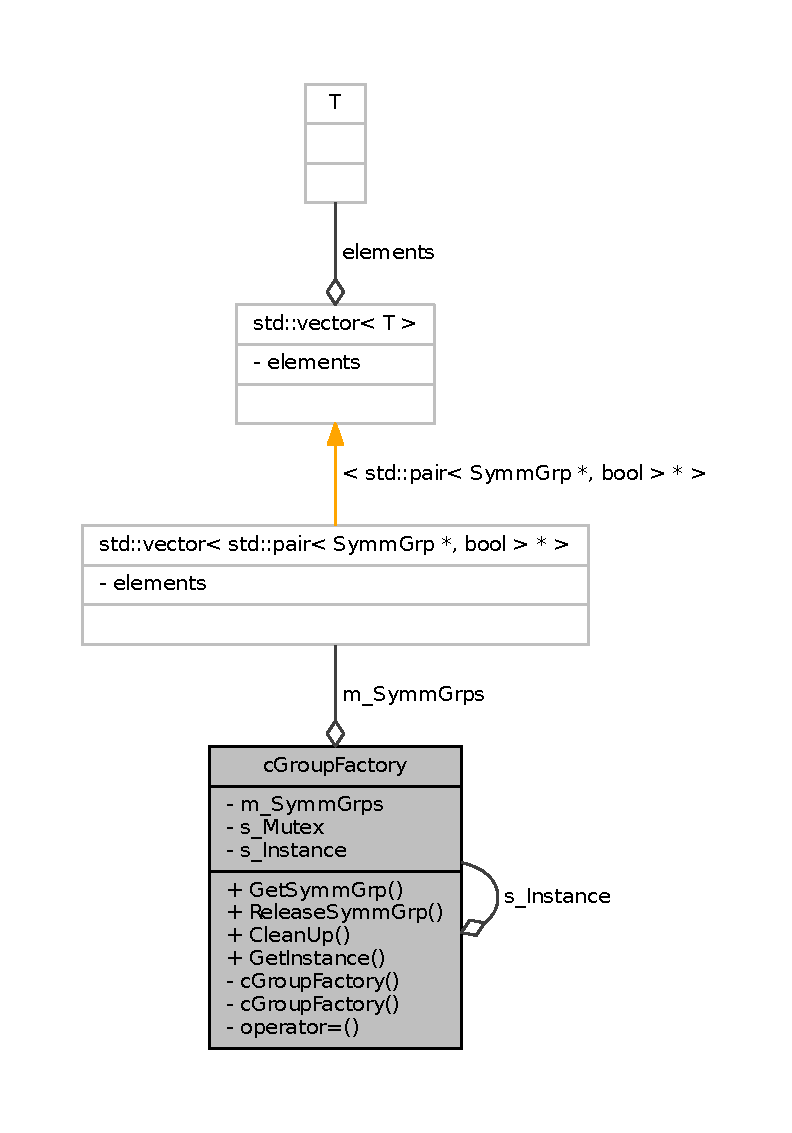
\includegraphics[width=280pt]{classcGroupFactory__coll__graph}
\end{center}
\end{figure}
\subsection*{Public Member Functions}
\begin{DoxyCompactItemize}
\item 
\hypertarget{classcGroupFactory_a079cb48ea3b9cf70b5c1af7537d5a2bb}{Symm\-Grp $\ast$ {\bfseries Get\-Symm\-Grp} (Symm\-Grp\-Elem \&generators)}\label{classcGroupFactory_a079cb48ea3b9cf70b5c1af7537d5a2bb}

\item 
\hypertarget{classcGroupFactory_a1f976090fb1ff95d94fca1eed602382d}{void {\bfseries Release\-Symm\-Grp} (Symm\-Grp $\ast$group)}\label{classcGroupFactory_a1f976090fb1ff95d94fca1eed602382d}

\item 
\hypertarget{classcGroupFactory_a1158bb4ce7d48072e10dc81c92739ae3}{void {\bfseries Clean\-Up} ()}\label{classcGroupFactory_a1158bb4ce7d48072e10dc81c92739ae3}

\end{DoxyCompactItemize}
\subsection*{Static Public Member Functions}
\begin{DoxyCompactItemize}
\item 
\hypertarget{classcGroupFactory_ae36952cd3999d331756a75a776e7a447}{static \hyperlink{classcGroupFactory}{c\-Group\-Factory} \& {\bfseries Get\-Instance} ()}\label{classcGroupFactory_ae36952cd3999d331756a75a776e7a447}

\end{DoxyCompactItemize}
\subsection*{Private Member Functions}
\begin{DoxyCompactItemize}
\item 
\hypertarget{classcGroupFactory_a7574dae0e4a358211ce79adf75a39ed2}{{\bfseries c\-Group\-Factory} (const \hyperlink{classcGroupFactory}{c\-Group\-Factory} \&grpfact)}\label{classcGroupFactory_a7574dae0e4a358211ce79adf75a39ed2}

\item 
\hypertarget{classcGroupFactory_a1c4edf0b35f3152a618f275bf459e7f3}{\hyperlink{classcGroupFactory}{c\-Group\-Factory} \& {\bfseries operator=} (\hyperlink{classcGroupFactory}{c\-Group\-Factory} \&grpfact)}\label{classcGroupFactory_a1c4edf0b35f3152a618f275bf459e7f3}

\end{DoxyCompactItemize}
\subsection*{Private Attributes}
\begin{DoxyCompactItemize}
\item 
\hypertarget{classcGroupFactory_a971617f9dd69295a27aede82781d3a8e}{std\-::vector$<$ std\-::pair\\*
$<$ Symm\-Grp $\ast$, bool $>$ $\ast$ $>$ {\bfseries m\-\_\-\-Symm\-Grps}}\label{classcGroupFactory_a971617f9dd69295a27aede82781d3a8e}

\end{DoxyCompactItemize}
\subsection*{Static Private Attributes}
\begin{DoxyCompactItemize}
\item 
\hypertarget{classcGroupFactory_abc9e8708326d158987ac8665b672be25}{static boost\-::mutex {\bfseries s\-\_\-\-Mutex}}\label{classcGroupFactory_abc9e8708326d158987ac8665b672be25}

\item 
\hypertarget{classcGroupFactory_aee9b5a04dd76633ef13aa16caa9ad310}{static \hyperlink{classcGroupFactory}{c\-Group\-Factory} $\ast$ {\bfseries s\-\_\-\-Instance}}\label{classcGroupFactory_aee9b5a04dd76633ef13aa16caa9ad310}

\end{DoxyCompactItemize}


\subsection{Detailed Description}
singleton class used to facilitate creation of groups contains a pool of groups for optimization 

The documentation for this class was generated from the following files\-:\begin{DoxyCompactItemize}
\item 
group\-\_\-factory.\-h\item 
group\-\_\-factory.\-cpp\end{DoxyCompactItemize}

\hypertarget{classengine_1_1cGroupGenCommand}{\section{engine\-:\-:c\-Group\-Gen\-Command Class Reference}
\label{classengine_1_1cGroupGenCommand}\index{engine\-::c\-Group\-Gen\-Command@{engine\-::c\-Group\-Gen\-Command}}
}


{\ttfamily \#include $<$groupgen\-\_\-command.\-h$>$}



Inheritance diagram for engine\-:\-:c\-Group\-Gen\-Command\-:


Collaboration diagram for engine\-:\-:c\-Group\-Gen\-Command\-:
\subsection*{Public Member Functions}
\begin{DoxyCompactItemize}
\item 
\hypertarget{classengine_1_1cGroupGenCommand_a94d3c632e772f19a07dfb15a4d46a0d4}{{\bfseries c\-Group\-Gen\-Command} (G\-R\-O\-U\-P\-\_\-\-T\-Y\-P\-E group\-\_\-type, const std\-::vector$<$ boost\-::any $>$ \&generators)}\label{classengine_1_1cGroupGenCommand_a94d3c632e772f19a07dfb15a4d46a0d4}

\item 
\hypertarget{classengine_1_1cGroupGenCommand_a37b02fb65826fa2bccc6ca071eec3c64}{const G\-R\-O\-U\-P\-\_\-\-T\-Y\-P\-E {\bfseries Get\-Group\-Type} () const }\label{classengine_1_1cGroupGenCommand_a37b02fb65826fa2bccc6ca071eec3c64}

\item 
\hypertarget{classengine_1_1cGroupGenCommand_a508e5a05d72dcfc34c1bb9859b901a97}{const std\-::vector$<$ Symm\-Grp\-Elem $>$ \& {\bfseries Get\-Result} () const }\label{classengine_1_1cGroupGenCommand_a508e5a05d72dcfc34c1bb9859b901a97}

\item 
\hypertarget{classengine_1_1cGroupGenCommand_a423b76a5c2dbf49db40655f968f15758}{const std\-::vector$<$ boost\-::any $>$ \& {\bfseries Get\-Generators} () const }\label{classengine_1_1cGroupGenCommand_a423b76a5c2dbf49db40655f968f15758}

\end{DoxyCompactItemize}
\subsection*{Protected Attributes}
\begin{DoxyCompactItemize}
\item 
\hypertarget{classengine_1_1cGroupGenCommand_ab878cfec34e06b0768f6efdbf9deb9fa}{G\-R\-O\-U\-P\-\_\-\-T\-Y\-P\-E {\bfseries m\-\_\-\-Grp\-Type}}\label{classengine_1_1cGroupGenCommand_ab878cfec34e06b0768f6efdbf9deb9fa}

\item 
\hypertarget{classengine_1_1cGroupGenCommand_acff9a3269f987eadf5b39412c09fe497}{std\-::vector$<$ boost\-::any $>$ {\bfseries m\-\_\-\-Generators}}\label{classengine_1_1cGroupGenCommand_acff9a3269f987eadf5b39412c09fe497}

\item 
\hypertarget{classengine_1_1cGroupGenCommand_a82938b2e1e2254bbecd5862d75025834}{std\-::vector$<$ Symm\-Grp\-Elem $>$ {\bfseries m\-\_\-\-Result}}\label{classengine_1_1cGroupGenCommand_a82938b2e1e2254bbecd5862d75025834}

\end{DoxyCompactItemize}


\subsection{Detailed Description}
holds data common to group commands 

The documentation for this class was generated from the following file\-:\begin{DoxyCompactItemize}
\item 
groupgen\-\_\-command.\-h\end{DoxyCompactItemize}

\hypertarget{classcInterpreter}{\section{c\-Interpreter Class Reference}
\label{classcInterpreter}\index{c\-Interpreter@{c\-Interpreter}}
}


Collaboration diagram for c\-Interpreter\-:


The documentation for this class was generated from the following file\-:\begin{DoxyCompactItemize}
\item 
interpreter.\-h\end{DoxyCompactItemize}

\hypertarget{classengine_1_1cLogger}{\section{engine\-:\-:c\-Logger \-Class \-Reference}
\label{classengine_1_1cLogger}\index{engine\-::c\-Logger@{engine\-::c\-Logger}}
}


\-Collaboration diagram for engine\-:\-:c\-Logger\-:
\nopagebreak
\begin{figure}[H]
\begin{center}
\leavevmode
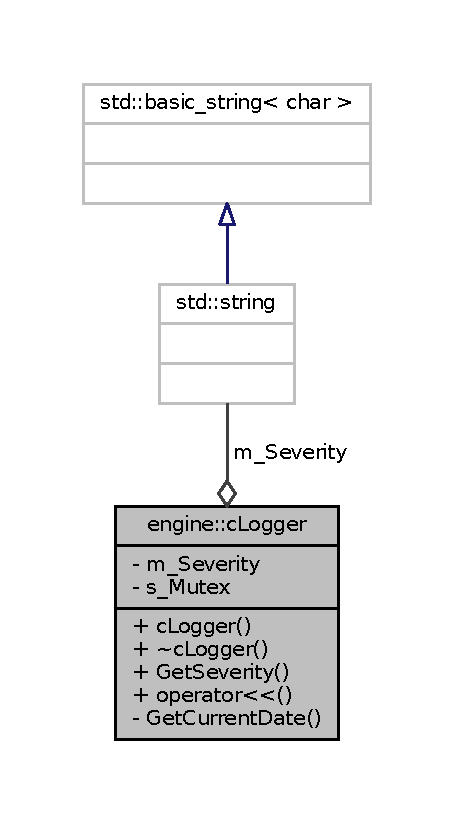
\includegraphics[width=218pt]{classengine_1_1cLogger__coll__graph}
\end{center}
\end{figure}
\subsection*{\-Public \-Member \-Functions}
\begin{DoxyCompactItemize}
\item 
\hypertarget{classengine_1_1cLogger_a127edc3f43400830cc8b46a1ccd5d183}{{\bfseries c\-Logger} (int severity)}\label{classengine_1_1cLogger_a127edc3f43400830cc8b46a1ccd5d183}

\item 
\hypertarget{classengine_1_1cLogger_a1473c1a79b0e677476da12f457fd8ff6}{const std\-::string \& {\bfseries \-Get\-Severity} () const }\label{classengine_1_1cLogger_a1473c1a79b0e677476da12f457fd8ff6}

\item 
\hypertarget{classengine_1_1cLogger_afaad3dca17bb3dd399d379e2ddd114b2}{\hyperlink{classengine_1_1cLogger}{c\-Logger} \& {\bfseries operator$<$$<$} (\-Supported\-Types type\-\_\-variant)}\label{classengine_1_1cLogger_afaad3dca17bb3dd399d379e2ddd114b2}

\end{DoxyCompactItemize}
\subsection*{\-Private \-Member \-Functions}
\begin{DoxyCompactItemize}
\item 
\hypertarget{classengine_1_1cLogger_a62d0c265a5fc3b81f8d31868edc34834}{std\-::string {\bfseries \-Get\-Current\-Date} () const }\label{classengine_1_1cLogger_a62d0c265a5fc3b81f8d31868edc34834}

\end{DoxyCompactItemize}
\subsection*{\-Private \-Attributes}
\begin{DoxyCompactItemize}
\item 
\hypertarget{classengine_1_1cLogger_a8214e9c0a088dbb98a4f4ea7ca9b9351}{std\-::string {\bfseries m\-\_\-\-Severity}}\label{classengine_1_1cLogger_a8214e9c0a088dbb98a4f4ea7ca9b9351}

\end{DoxyCompactItemize}
\subsection*{\-Static \-Private \-Attributes}
\begin{DoxyCompactItemize}
\item 
\hypertarget{classengine_1_1cLogger_a5276c31bbf002c5a224095504bac62c5}{static boost\-::mutex {\bfseries s\-\_\-\-Mutex}}\label{classengine_1_1cLogger_a5276c31bbf002c5a224095504bac62c5}

\end{DoxyCompactItemize}


\-The documentation for this class was generated from the following files\-:\begin{DoxyCompactItemize}
\item 
logger.\-h\item 
logger.\-cpp\end{DoxyCompactItemize}

\hypertarget{classengine_1_1cResult}{
\section{engine\-:\-:c\-Result \-Class \-Reference}
\label{classengine_1_1cResult}\index{engine\-::c\-Result@{engine\-::c\-Result}}
}


\-Collaboration diagram for engine\-:\-:c\-Result\-:\nopagebreak
\begin{figure}[H]
\begin{center}
\leavevmode
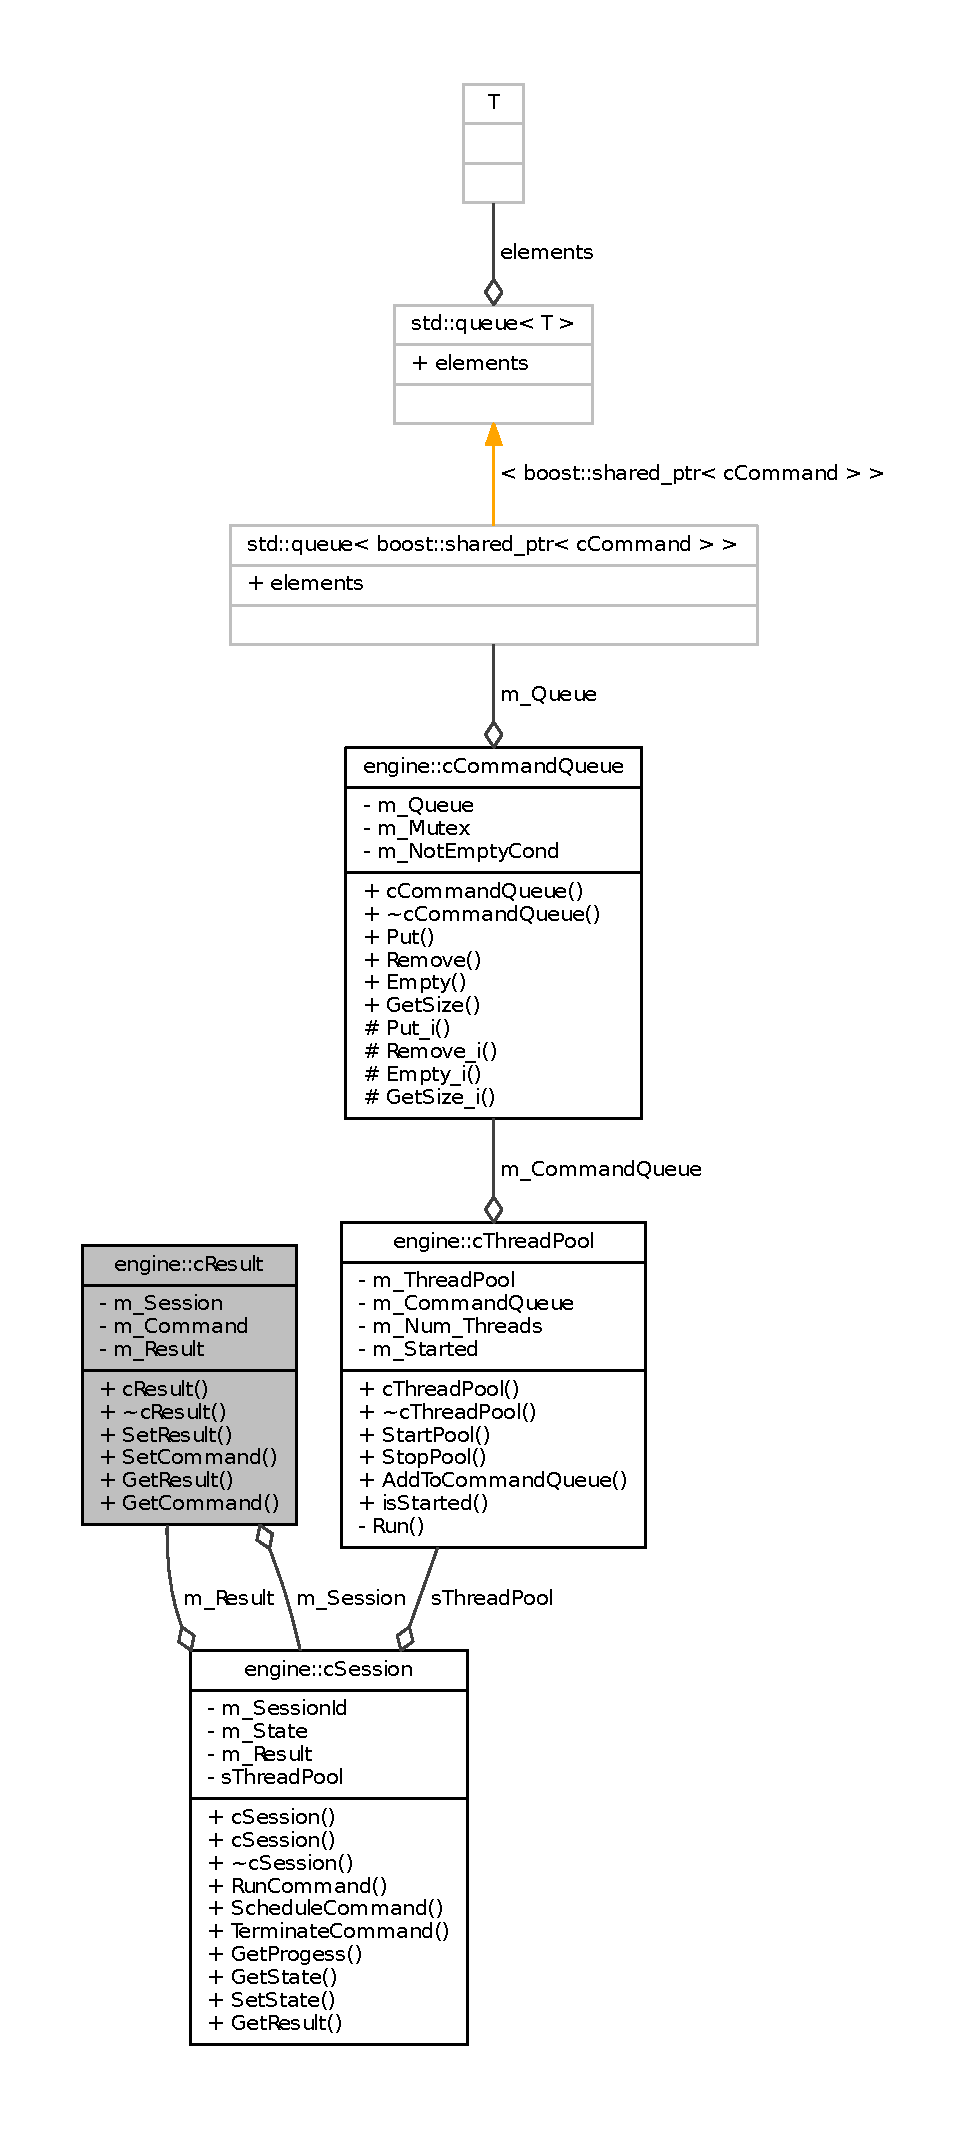
\includegraphics[height=550pt]{classengine_1_1cResult__coll__graph}
\end{center}
\end{figure}
\subsection*{\-Public \-Member \-Functions}
\begin{DoxyCompactItemize}
\item 
\hypertarget{classengine_1_1cResult_a31310dd255e30fdaeb34aa0e82c489f3}{
{\bfseries c\-Result} (\hyperlink{classengine_1_1cSession}{c\-Session} $\ast$session=\-N\-U\-L\-L, \hyperlink{classengine_1_1cCommand}{c\-Command} $\ast$command=\-N\-U\-L\-L)}
\label{classengine_1_1cResult_a31310dd255e30fdaeb34aa0e82c489f3}

\item 
\hypertarget{classengine_1_1cResult_ad72c10e84728768e45adbe9a653e4295}{
void {\bfseries \-Set\-Result} (const boost\-::any \&result)}
\label{classengine_1_1cResult_ad72c10e84728768e45adbe9a653e4295}

\item 
\hypertarget{classengine_1_1cResult_ae9d0c2817585874e55a9ba8483e9d0b7}{
void {\bfseries \-Set\-Command} (\hyperlink{classengine_1_1cCommand}{c\-Command} $\ast$command)}
\label{classengine_1_1cResult_ae9d0c2817585874e55a9ba8483e9d0b7}

\item 
\hypertarget{classengine_1_1cResult_ab1b5a9a971a31c6bfe9c1deeab868476}{
const boost\-::any \& {\bfseries \-Get\-Result} () const }
\label{classengine_1_1cResult_ab1b5a9a971a31c6bfe9c1deeab868476}

\item 
\hypertarget{classengine_1_1cResult_aa414e0f8b867fa54c6e836f0a67517b0}{
const \hyperlink{classengine_1_1cCommand}{c\-Command} $\ast$ {\bfseries \-Get\-Command} () const }
\label{classengine_1_1cResult_aa414e0f8b867fa54c6e836f0a67517b0}

\end{DoxyCompactItemize}
\subsection*{\-Private \-Attributes}
\begin{DoxyCompactItemize}
\item 
\hypertarget{classengine_1_1cResult_ab4a2a6e829775978c141dc4f18398321}{
\hyperlink{classengine_1_1cSession}{c\-Session} $\ast$ {\bfseries m\-\_\-\-Session}}
\label{classengine_1_1cResult_ab4a2a6e829775978c141dc4f18398321}

\item 
\hypertarget{classengine_1_1cResult_ae5500a8cd5d5c860c9c3c71a9bd687f1}{
\hyperlink{classengine_1_1cCommand}{c\-Command} $\ast$ {\bfseries m\-\_\-\-Command}}
\label{classengine_1_1cResult_ae5500a8cd5d5c860c9c3c71a9bd687f1}

\item 
\hypertarget{classengine_1_1cResult_a445a8b5495ec68e809fe85b5876a5bc7}{
boost\-::any {\bfseries m\-\_\-\-Result}}
\label{classengine_1_1cResult_a445a8b5495ec68e809fe85b5876a5bc7}

\end{DoxyCompactItemize}


\-The documentation for this class was generated from the following files\-:\begin{DoxyCompactItemize}
\item 
result.\-h\item 
result.\-cpp\end{DoxyCompactItemize}

\hypertarget{classcSerializer_3_01SymmGrpElem_00_01CONT_01_4}{\section{c\-Serializer$<$ \-Symm\-Grp\-Elem, \-C\-O\-N\-T $>$ \-Class \-Template \-Reference}
\label{classcSerializer_3_01SymmGrpElem_00_01CONT_01_4}\index{c\-Serializer$<$ Symm\-Grp\-Elem, C\-O\-N\-T $>$@{c\-Serializer$<$ Symm\-Grp\-Elem, C\-O\-N\-T $>$}}
}
\subsection*{\-Public \-Member \-Functions}
\begin{DoxyCompactItemize}
\item 
\hypertarget{classcSerializer_3_01SymmGrpElem_00_01CONT_01_4_a9f2b83d7cb75cfad5bd2a1c15fa968c1}{const std\-::string {\bfseries \-Stringify} (const \-Symm\-Grp\-Elem \&element) const }\label{classcSerializer_3_01SymmGrpElem_00_01CONT_01_4_a9f2b83d7cb75cfad5bd2a1c15fa968c1}

\item 
\hypertarget{classcSerializer_3_01SymmGrpElem_00_01CONT_01_4_adc87f8732b096f7add2f18f486bada73}{const std\-::string {\bfseries \-Stringify} (const \-C\-O\-N\-T$<$ \-Symm\-Grp\-Elem, std\-::allocator$<$ \-Symm\-Grp\-Elem $>$ $>$ \&elements) const }\label{classcSerializer_3_01SymmGrpElem_00_01CONT_01_4_adc87f8732b096f7add2f18f486bada73}

\end{DoxyCompactItemize}
\subsubsection*{template$<$template$<$ typename, class $>$ class \-C\-O\-N\-T$>$ class c\-Serializer$<$ Symm\-Grp\-Elem, C\-O\-N\-T $>$}



\-The documentation for this class was generated from the following file\-:\begin{DoxyCompactItemize}
\item 
serializer.\-h\end{DoxyCompactItemize}

\hypertarget{classengine_1_1cSession}{
\section{engine\-:\-:c\-Session \-Class \-Reference}
\label{classengine_1_1cSession}\index{engine\-::c\-Session@{engine\-::c\-Session}}
}


\-Collaboration diagram for engine\-:\-:c\-Session\-:\nopagebreak
\begin{figure}[H]
\begin{center}
\leavevmode
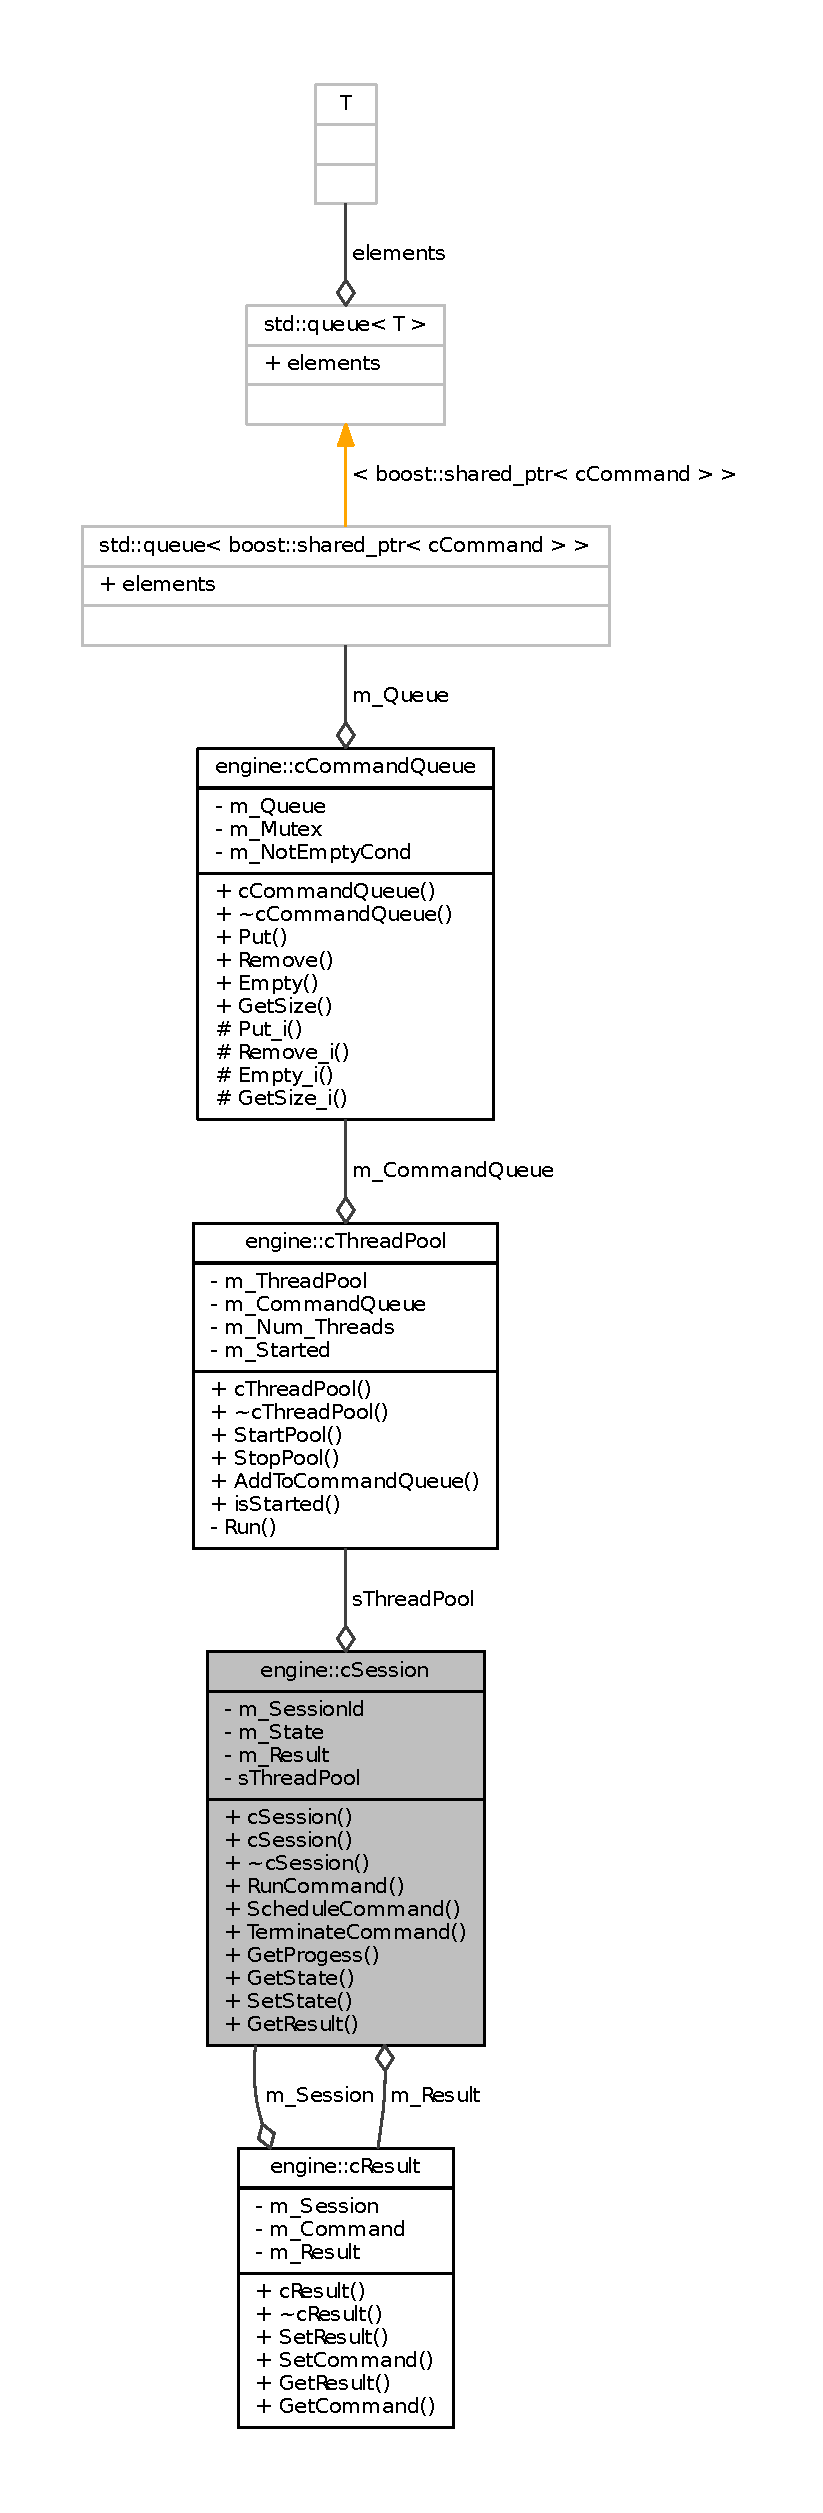
\includegraphics[height=550pt]{classengine_1_1cSession__coll__graph}
\end{center}
\end{figure}
\subsection*{\-Public \-Member \-Functions}
\begin{DoxyCompactItemize}
\item 
\hypertarget{classengine_1_1cSession_aafe0e5fd946fd5fa5b990617f848a5a5}{
{\bfseries c\-Session} (unsigned int ses\-\_\-id)}
\label{classengine_1_1cSession_aafe0e5fd946fd5fa5b990617f848a5a5}

\item 
\hypertarget{classengine_1_1cSession_a79226f269db0a276764656791d7689f2}{
void {\bfseries \-Run\-Command} (\hyperlink{classengine_1_1cCommand}{c\-Command} $\ast$command)}
\label{classengine_1_1cSession_a79226f269db0a276764656791d7689f2}

\item 
\hypertarget{classengine_1_1cSession_afcf61cec37829291b2aa8e13d2ca96e0}{
void {\bfseries \-Schedule\-Command} (\hyperlink{classengine_1_1cCommand}{c\-Command} $\ast$command)}
\label{classengine_1_1cSession_afcf61cec37829291b2aa8e13d2ca96e0}

\item 
\hypertarget{classengine_1_1cSession_af1a1747cd7020bd4bfce782bf1ffec5d}{
void {\bfseries \-Terminate\-Command} ()}
\label{classengine_1_1cSession_af1a1747cd7020bd4bfce782bf1ffec5d}

\item 
\hypertarget{classengine_1_1cSession_ab5b73d57f8d6fd918d33b4e0a64c21d9}{
unsigned int {\bfseries \-Get\-Progess} ()}
\label{classengine_1_1cSession_ab5b73d57f8d6fd918d33b4e0a64c21d9}

\item 
\hypertarget{classengine_1_1cSession_a4d5cfbd1a1a5d1ff022fd4915b256f4f}{
int {\bfseries \-Get\-State} () const }
\label{classengine_1_1cSession_a4d5cfbd1a1a5d1ff022fd4915b256f4f}

\item 
\hypertarget{classengine_1_1cSession_ac70dfa95b25fed14a6ca32df68cf1300}{
void {\bfseries \-Set\-State} (int state)}
\label{classengine_1_1cSession_ac70dfa95b25fed14a6ca32df68cf1300}

\item 
\hypertarget{classengine_1_1cSession_aa403617485890fe288c5cf68b39ab540}{
\hyperlink{classengine_1_1cResult}{c\-Result} $\ast$ {\bfseries \-Get\-Result} ()}
\label{classengine_1_1cSession_aa403617485890fe288c5cf68b39ab540}

\end{DoxyCompactItemize}
\subsection*{\-Private \-Attributes}
\begin{DoxyCompactItemize}
\item 
\hypertarget{classengine_1_1cSession_a4adc27ebd913c027b736e9aa2f4142cb}{
int {\bfseries m\-\_\-\-Session\-Id}}
\label{classengine_1_1cSession_a4adc27ebd913c027b736e9aa2f4142cb}

\item 
\hypertarget{classengine_1_1cSession_af0edf0e0ced62ee7e8a5136637cc0084}{
volatile int {\bfseries m\-\_\-\-State}}
\label{classengine_1_1cSession_af0edf0e0ced62ee7e8a5136637cc0084}

\item 
\hypertarget{classengine_1_1cSession_abfc019aab8f8453fd7589266c0e00ef7}{
\hyperlink{classengine_1_1cResult}{c\-Result} {\bfseries m\-\_\-\-Result}}
\label{classengine_1_1cSession_abfc019aab8f8453fd7589266c0e00ef7}

\end{DoxyCompactItemize}
\subsection*{\-Static \-Private \-Attributes}
\begin{DoxyCompactItemize}
\item 
\hypertarget{classengine_1_1cSession_a2f0a00f5302fdf8d88d4738c448ce4fa}{
static \hyperlink{classengine_1_1cThreadPool}{c\-Thread\-Pool} {\bfseries s\-Thread\-Pool}}
\label{classengine_1_1cSession_a2f0a00f5302fdf8d88d4738c448ce4fa}

\end{DoxyCompactItemize}


\-The documentation for this class was generated from the following files\-:\begin{DoxyCompactItemize}
\item 
session.\-h\item 
session.\-cpp\end{DoxyCompactItemize}

\hypertarget{classengine_1_1cThreadPool}{\section{engine\-:\-:c\-Thread\-Pool \-Class \-Reference}
\label{classengine_1_1cThreadPool}\index{engine\-::c\-Thread\-Pool@{engine\-::c\-Thread\-Pool}}
}


{\ttfamily \#include $<$thread\-\_\-pool.\-h$>$}



\-Collaboration diagram for engine\-:\-:c\-Thread\-Pool\-:\nopagebreak
\begin{figure}[H]
\begin{center}
\leavevmode
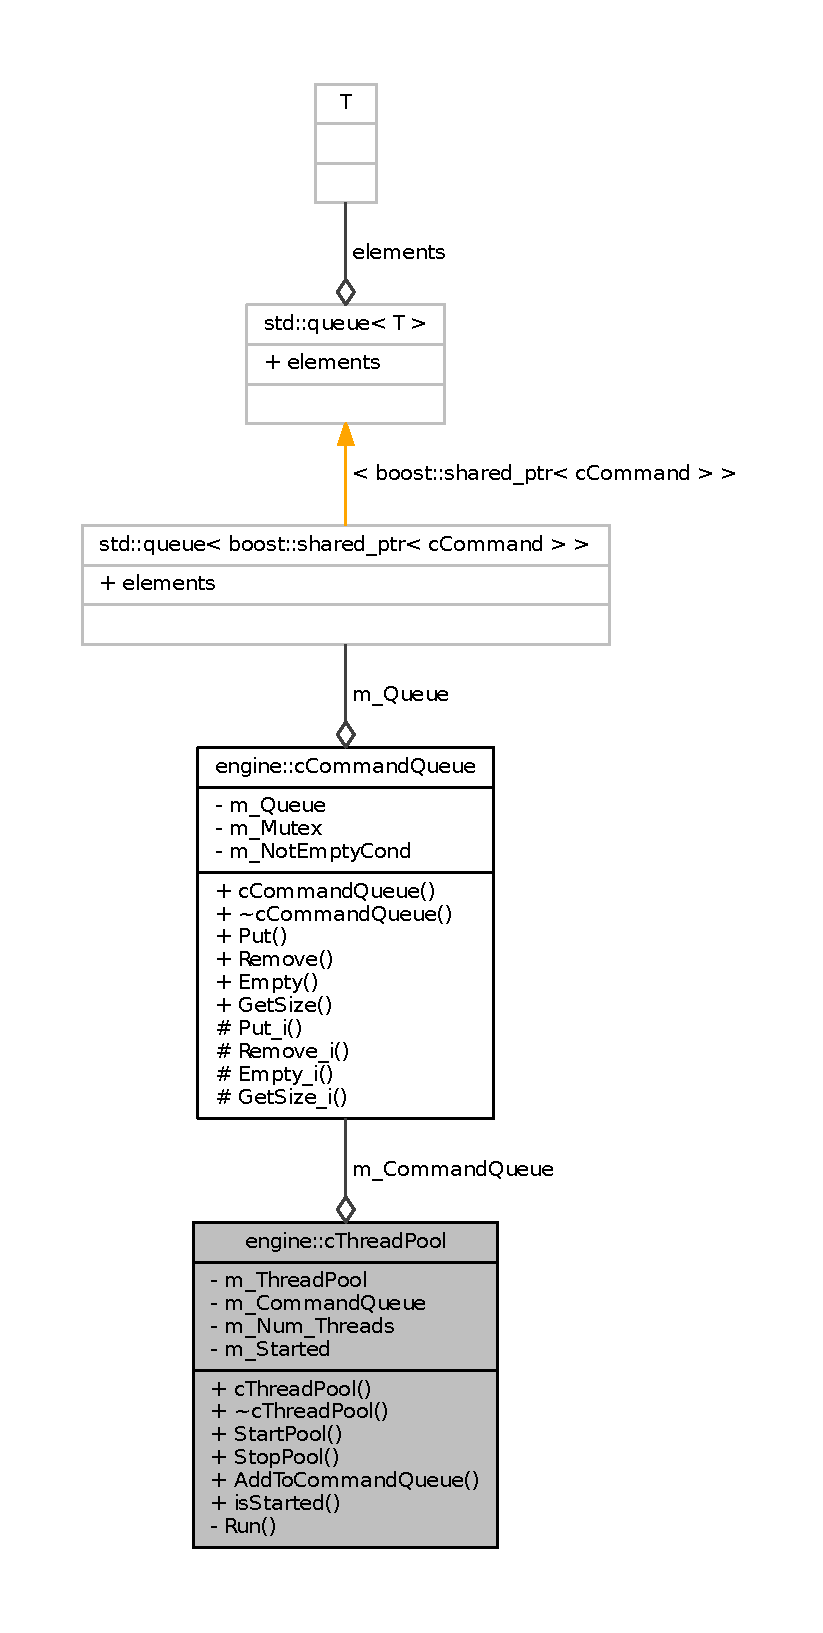
\includegraphics[height=550pt]{classengine_1_1cThreadPool__coll__graph}
\end{center}
\end{figure}
\subsection*{\-Public \-Member \-Functions}
\begin{DoxyCompactItemize}
\item 
\hypertarget{classengine_1_1cThreadPool_a1cef23416a63c1a652d07b074a40b42e}{{\bfseries c\-Thread\-Pool} (unsigned int num\-\_\-threads)}\label{classengine_1_1cThreadPool_a1cef23416a63c1a652d07b074a40b42e}

\item 
\hypertarget{classengine_1_1cThreadPool_a97cf0269aebd226e59d973a89181d709}{void {\bfseries \-Start\-Pool} ()}\label{classengine_1_1cThreadPool_a97cf0269aebd226e59d973a89181d709}

\item 
\hypertarget{classengine_1_1cThreadPool_aeafab9fa5546e10b0deebff1e8df60d9}{void {\bfseries \-Stop\-Pool} ()}\label{classengine_1_1cThreadPool_aeafab9fa5546e10b0deebff1e8df60d9}

\item 
\hypertarget{classengine_1_1cThreadPool_a0c20020f1a69f4ea0abdb75d1adde225}{void {\bfseries \-Add\-To\-Command\-Queue} (\hyperlink{classengine_1_1cCommand}{c\-Command} $\ast$command)}\label{classengine_1_1cThreadPool_a0c20020f1a69f4ea0abdb75d1adde225}

\item 
\hypertarget{classengine_1_1cThreadPool_a207b8bcf506d3cd151f0fc815772111c}{bool {\bfseries is\-Started} () const }\label{classengine_1_1cThreadPool_a207b8bcf506d3cd151f0fc815772111c}

\end{DoxyCompactItemize}
\subsection*{\-Private \-Member \-Functions}
\begin{DoxyCompactItemize}
\item 
void \hyperlink{classengine_1_1cThreadPool_af573f11026d6b6079c56af7e50df5ca6}{\-Run} ()
\end{DoxyCompactItemize}
\subsection*{\-Private \-Attributes}
\begin{DoxyCompactItemize}
\item 
\hypertarget{classengine_1_1cThreadPool_ae0439f245252951c72e929fcb5f12ea7}{boost\-::thread\-\_\-group {\bfseries m\-\_\-\-Thread\-Pool}}\label{classengine_1_1cThreadPool_ae0439f245252951c72e929fcb5f12ea7}

\item 
\hypertarget{classengine_1_1cThreadPool_a9e8295a610871d54220f068d447e4b3d}{\hyperlink{classengine_1_1cCommandQueue}{c\-Command\-Queue} {\bfseries m\-\_\-\-Command\-Queue}}\label{classengine_1_1cThreadPool_a9e8295a610871d54220f068d447e4b3d}

\item 
\hypertarget{classengine_1_1cThreadPool_a5a9ba1d9f84c6edf6312c358973c1e75}{volatile unsigned int {\bfseries m\-\_\-\-Num\-\_\-\-Threads}}\label{classengine_1_1cThreadPool_a5a9ba1d9f84c6edf6312c358973c1e75}

\item 
\hypertarget{classengine_1_1cThreadPool_a665b990bbfe85aa6dd9be2691373e2d7}{volatile bool {\bfseries m\-\_\-\-Started}}\label{classengine_1_1cThreadPool_a665b990bbfe85aa6dd9be2691373e2d7}

\end{DoxyCompactItemize}


\subsection{\-Detailed \-Description}
thread pool class uses a queue to hold the commands received 

\subsection{\-Member \-Function \-Documentation}
\hypertarget{classengine_1_1cThreadPool_af573f11026d6b6079c56af7e50df5ca6}{\index{engine\-::c\-Thread\-Pool@{engine\-::c\-Thread\-Pool}!\-Run@{\-Run}}
\index{\-Run@{\-Run}!engine::cThreadPool@{engine\-::c\-Thread\-Pool}}
\subsubsection[{\-Run}]{\setlength{\rightskip}{0pt plus 5cm}void {\bf engine\-::c\-Thread\-Pool\-::\-Run} (
\begin{DoxyParamCaption}
{}
\end{DoxyParamCaption}
)\hspace{0.3cm}{\ttfamily  \mbox{[}private\mbox{]}}}}\label{classengine_1_1cThreadPool_af573f11026d6b6079c56af7e50df5ca6}
function that runs in all the threads waits until the queue is not empty and process incoming commands 

\-The documentation for this class was generated from the following files\-:\begin{DoxyCompactItemize}
\item 
thread\-\_\-pool.\-h\item 
thread\-\_\-pool.\-cpp\end{DoxyCompactItemize}

\hypertarget{classengine_1_1cVariantVisitor}{\section{engine\-:\-:c\-Variant\-Visitor Class Reference}
\label{classengine_1_1cVariantVisitor}\index{engine\-::c\-Variant\-Visitor@{engine\-::c\-Variant\-Visitor}}
}


Inheritance diagram for engine\-:\-:c\-Variant\-Visitor\-:
\nopagebreak
\begin{figure}[H]
\begin{center}
\leavevmode
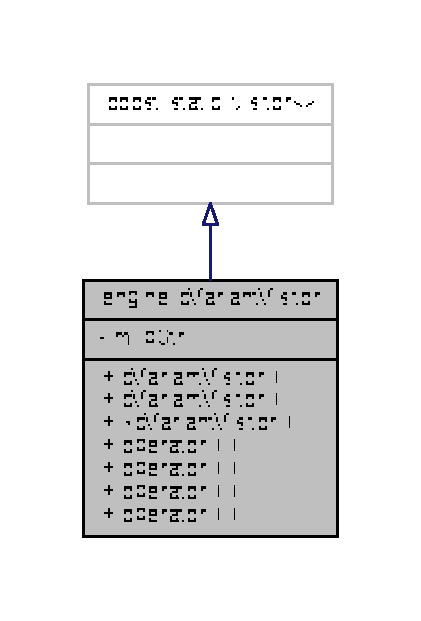
\includegraphics[width=202pt]{classengine_1_1cVariantVisitor__inherit__graph}
\end{center}
\end{figure}


Collaboration diagram for engine\-:\-:c\-Variant\-Visitor\-:
\nopagebreak
\begin{figure}[H]
\begin{center}
\leavevmode
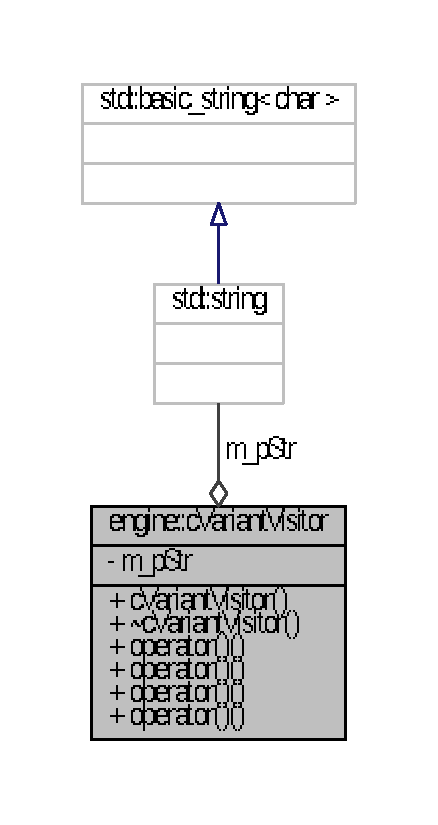
\includegraphics[width=295pt]{classengine_1_1cVariantVisitor__coll__graph}
\end{center}
\end{figure}
\subsection*{Public Member Functions}
\begin{DoxyCompactItemize}
\item 
\hypertarget{classengine_1_1cVariantVisitor_a4dfcf482b3b84120ab323aa9303058f0}{{\bfseries c\-Variant\-Visitor} (std\-::string $\ast$str)}\label{classengine_1_1cVariantVisitor_a4dfcf482b3b84120ab323aa9303058f0}

\item 
\hypertarget{classengine_1_1cVariantVisitor_ab49278c7d44ba02e5a411063cb5e5593}{{\bfseries c\-Variant\-Visitor} (const \hyperlink{classengine_1_1cVariantVisitor}{c\-Variant\-Visitor} \&var\-\_\-vis)}\label{classengine_1_1cVariantVisitor_ab49278c7d44ba02e5a411063cb5e5593}

\item 
\hypertarget{classengine_1_1cVariantVisitor_a194e92aa8a44b02c29dbe14a5a049493}{void {\bfseries operator()} (const int \&integer)}\label{classengine_1_1cVariantVisitor_a194e92aa8a44b02c29dbe14a5a049493}

\item 
\hypertarget{classengine_1_1cVariantVisitor_ad72499c182f11280fa498773ffc8bd3c}{void {\bfseries operator()} (const double \&real\-\_\-num)}\label{classengine_1_1cVariantVisitor_ad72499c182f11280fa498773ffc8bd3c}

\item 
\hypertarget{classengine_1_1cVariantVisitor_a1f1bc8f29028034cddb07f1781e56e81}{void {\bfseries operator()} (const std\-::exception \&exception)}\label{classengine_1_1cVariantVisitor_a1f1bc8f29028034cddb07f1781e56e81}

\item 
\hypertarget{classengine_1_1cVariantVisitor_afdfa31a083e06c49529beeea2557dce4}{void {\bfseries operator()} (const std\-::string \&message)}\label{classengine_1_1cVariantVisitor_afdfa31a083e06c49529beeea2557dce4}

\end{DoxyCompactItemize}
\subsection*{Private Attributes}
\begin{DoxyCompactItemize}
\item 
\hypertarget{classengine_1_1cVariantVisitor_a0392f224211e16af4b2c72afa2df4257}{std\-::string $\ast$ {\bfseries m\-\_\-p\-Str}}\label{classengine_1_1cVariantVisitor_a0392f224211e16af4b2c72afa2df4257}

\end{DoxyCompactItemize}


\subsection{Detailed Description}
class implementing the strategy pattern in order interpret different types of objects as errors 

The documentation for this class was generated from the following file\-:\begin{DoxyCompactItemize}
\item 
logger.\-cpp\end{DoxyCompactItemize}

\hypertarget{structengine_1_1cGroupGenCommand_1_1group__type__}{
\section{engine\-:\-:c\-Group\-Gen\-Command\-:\-:group\-\_\-type\-\_\- \-Struct \-Reference}
\label{structengine_1_1cGroupGenCommand_1_1group__type__}\index{engine\-::c\-Group\-Gen\-Command\-::group\-\_\-type\-\_\-@{engine\-::c\-Group\-Gen\-Command\-::group\-\_\-type\-\_\-}}
}


\-The documentation for this struct was generated from the following file\-:\begin{DoxyCompactItemize}
\item 
groupgen\-\_\-command.\-h\end{DoxyCompactItemize}

\printindex
\end{document}
